\documentclass[dvipdfmx]{jsarticle}
\setcounter{section}{1}
\setcounter{subsection}{4}
\usepackage{xr}
\externaldocument{2.1.2}
\externaldocument{2.1.4}
\usepackage{amsmath,amsfonts,amssymb,array,comment,mathtools,url,docmute}
\usepackage{longtable,booktabs,dcolumn,tabularx,mathtools,multirow,colortbl,xcolor}
\usepackage[dvipdfmx]{graphics}
\usepackage{bmpsize}
\usepackage{amsthm}
\usepackage{enumitem}
\setlistdepth{20}
\renewlist{itemize}{itemize}{20}
\setlist[itemize]{label=•}
\renewlist{enumerate}{enumerate}{20}
\setlist[enumerate]{label=\arabic*.}
\setcounter{MaxMatrixCols}{20}
\setcounter{tocdepth}{3}
\newcommand{\rotin}{\text{\rotatebox[origin=c]{90}{$\in $}}}
\newcommand{\amap}[6]{\text{\raisebox{-0.7cm}{\begin{tikzpicture} 
  \node (a) at (0, 1) {$\textstyle{#2}$};
  \node (b) at (#6, 1) {$\textstyle{#3}$};
  \node (c) at (0, 0) {$\textstyle{#4}$};
  \node (d) at (#6, 0) {$\textstyle{#5}$};
  \node (x) at (0, 0.5) {$\rotin $};
  \node (x) at (#6, 0.5) {$\rotin $};
  \draw[->] (a) to node[xshift=0pt, yshift=7pt] {$\textstyle{\scriptstyle{#1}}$} (b);
  \draw[|->] (c) to node[xshift=0pt, yshift=7pt] {$\textstyle{\scriptstyle{#1}}$} (d);
\end{tikzpicture}}}}
\newcommand{\twomaps}[9]{\text{\raisebox{-0.7cm}{\begin{tikzpicture} 
  \node (a) at (0, 1) {$\textstyle{#3}$};
  \node (b) at (#9, 1) {$\textstyle{#4}$};
  \node (c) at (#9+#9, 1) {$\textstyle{#5}$};
  \node (d) at (0, 0) {$\textstyle{#6}$};
  \node (e) at (#9, 0) {$\textstyle{#7}$};
  \node (f) at (#9+#9, 0) {$\textstyle{#8}$};
  \node (x) at (0, 0.5) {$\rotin $};
  \node (x) at (#9, 0.5) {$\rotin $};
  \node (x) at (#9+#9, 0.5) {$\rotin $};
  \draw[->] (a) to node[xshift=0pt, yshift=7pt] {$\textstyle{\scriptstyle{#1}}$} (b);
  \draw[|->] (d) to node[xshift=0pt, yshift=7pt] {$\textstyle{\scriptstyle{#2}}$} (e);
  \draw[->] (b) to node[xshift=0pt, yshift=7pt] {$\textstyle{\scriptstyle{#1}}$} (c);
  \draw[|->] (e) to node[xshift=0pt, yshift=7pt] {$\textstyle{\scriptstyle{#2}}$} (f);
\end{tikzpicture}}}}
\renewcommand{\thesection}{第\arabic{section}部}
\renewcommand{\thesubsection}{\arabic{section}.\arabic{subsection}}
\renewcommand{\thesubsubsection}{\arabic{section}.\arabic{subsection}.\arabic{subsubsection}}
\everymath{\displaystyle}
\allowdisplaybreaks[4]
\usepackage{vtable}
\theoremstyle{definition}
\newtheorem{thm}{定理}[subsection]
\newtheorem*{thm*}{定理}
\newtheorem{dfn}{定義}[subsection]
\newtheorem*{dfn*}{定義}
\newtheorem{axs}[dfn]{公理}
\newtheorem*{axs*}{公理}
\renewcommand{\headfont}{\bfseries}
\makeatletter
  \renewcommand{\section}{%
    \@startsection{section}{1}{\z@}%
    {\Cvs}{\Cvs}%
    {\normalfont\huge\headfont\raggedright}}
\makeatother
\makeatletter
  \renewcommand{\subsection}{%
    \@startsection{subsection}{2}{\z@}%
    {0.5\Cvs}{0.5\Cvs}%
    {\normalfont\LARGE\headfont\raggedright}}
\makeatother
\makeatletter
  \renewcommand{\subsubsection}{%
    \@startsection{subsubsection}{3}{\z@}%
    {0.4\Cvs}{0.4\Cvs}%
    {\normalfont\Large\headfont\raggedright}}
\makeatother
\makeatletter
\renewenvironment{proof}[1][\proofname]{\par
  \pushQED{\qed}%
  \normalfont \topsep6\p@\@plus6\p@\relax
  \trivlist
  \item\relax
  {
  #1\@addpunct{.}}\hspace\labelsep\ignorespaces
}{%
  \popQED\endtrivlist\@endpefalse
}
\makeatother
\renewcommand{\proofname}{\textbf{証明}}
\usepackage{tikz,graphics}
\usepackage[dvipdfmx]{hyperref}
\usepackage{pxjahyper}
\hypersetup{
 setpagesize=false,
 bookmarks=true,
 bookmarksdepth=tocdepth,
 bookmarksnumbered=true,
 colorlinks=false,
 pdftitle={},
 pdfsubject={},
 pdfauthor={},
 pdfkeywords={}}
\begin{document}
%\hypertarget{ux8868ux73feux884cux5217}{%
\subsection{表現行列}%\label{ux8868ux73feux884cux5217}}
%\hypertarget{ux7ddaux5f62ux5199ux50cf}{%
\subsubsection{線形写像}%\label{ux7ddaux5f62ux5199ux50cf}}
\begin{dfn*}[定義\ref{線形写像}の再掲]
体$K$上のvector空間$V$、$W$において写像$f:V \rightarrow W$が、$\forall\mathbf{v},\mathbf{w} \in V\forall k,l \in K$に対し、$f\left( k\mathbf{v} + l\mathbf{w} \right) = kf\left( \mathbf{v} \right) + lf\left( \mathbf{w} \right)$を満たすとき、この写像を体$K$上のvector空間として準同型写像、体$K$上のvector空間$V$から$W$への線形写像、体$K$上で線形的な写像などという。体$K$はvector空間が満たすべき条件が揃っているので、体$K$上のvector空間$V$から体$K$への線形写像を特にvector空間$V$の線形形式という。
\end{dfn*}\par
以下ここでは、今まで扱ってきた概念たちが挙げられよう。
\begin{dfn*}[定義\ref{線形同型写像}の再掲]
体$K$上の2つのvector空間たち$V$、$W$が与えられたとする。線形写像$f:V \rightarrow W$が全単射であるとき、この写像$f$をその体$K$上のそのvector空間$V$からそのvector空間$W$への線形同型写像、同型写像などといい、その体$K$上のそのvector空間$V$からそのvector空間$W$への線形同型写像が存在するとき、そのvector空間$V$とそのvector空間$W$は線形同型であるなどといい$V \cong W$などと書く。
\end{dfn*}\par
もちろん、そのvector空間$V$の恒等写像$I_{V}もV$の線形自己同型写像である。
\begin{dfn*}[定義\ref{線形写像の像と核}の再掲]
体$K$上の2つのvector空間$V$、$W$を用いて線形写像$f:V \rightarrow W$が与えられたとき、次式のような集合$V(f)$をその写像$f$の値域、像といい$f(V)$、$\mathrm{Im}f$などと書く。
\begin{align*}
V(f) = \left\{ f\left( \mathbf{v} \right) \in W|\mathbf{v} \in V \right\} \subseteq W
\end{align*}
また、次式のような集合、即ち、$f\left( \mathbf{v} \right) = \mathbf{0}$となるようなvector空間$V$の元$\mathbf{v}$全体の集合で写像$f$を対応とみなしたときの逆対応$f^{- 1}$に$\mathbf{v} = \mathbf{0}$とした像をその写像$f$の核といい、$\ker_{K}f$、$\ker f$などと書く。
\end{dfn*}
\begin{dfn*}[定義\ref{線形写像の階数と退化次数}の再掲]
体$K$上の2つのvector空間$V$、$W$を用いて線形写像$f:V \rightarrow W$が与えられたとき、その写像$f$の値域$V(f)$の次元$\dim{V(f)}$をその写像$f$の階数、その核$\ker f$の次元$\dim{\ker f}$をその写像$f$の退化次数といいそれぞれ${\mathrm{rank}}f$、${\mathrm{nullity}}f$と書く。
\end{dfn*}
\begin{thm*}[次元公式\ref{2.1.2.14}の再掲]
体$K$上の2つのvector空間$V$、$W$を用いた線形写像$f:V \rightarrow W$が与えられ、そのvector空間$V$が有限次元であるとき、次式が成り立つ。
\begin{align*}
{\mathrm{rank}}f + {\mathrm{nullity}}f = \dim{V(f)} + \dim{\ker f} = \dim V
\end{align*}
この式、または、この定理を次元公式という。
\end{thm*}
\begin{thm*}[定理\ref{2.1.4.15}の再掲]
集合$M_{nn}(K)$に属する$n$次正方行列$A_{nn}$について、次のことは同値である。
\begin{itemize}
\item
  線形写像$L_{A_{nn}}:K^{n} \rightarrow K^{n};\mathbf{v} \mapsto A_{nn}\mathbf{v}$が全単射である。
\item
  ${\mathrm{rank}}A_{nn} = n$が成り立つ。
\item
  $\exists A_{nn}^{- 1} \in M_{nn}(K)$に対し、$A_{nn}A_{nn}^{- 1} = A_{nn}^{- 1}A_{nn} = I_{n}$が成り立つ。
\item
  $\ker L_{A_{mn}} = \left\{ \mathbf{0} \right\}$が成り立つ。
\item
  $\forall\mathbf{v} \in K^{n}$に対し、$A_{nn}\mathbf{v} = \mathbf{0}$が成り立つならそのときに限り、$\mathbf{v} = \mathbf{0}$が成り立つ。
\end{itemize}
\end{thm*}
\begin{dfn*}[定義\ref{正則行列}の再掲]
$n$次正方行列$A_{nn}$が上の条件たちのうち少なくとも1つ満たせば、その他全ての条件たちを満たす。このような行列$A_{nn}$を正則行列などといいこのような行列$A_{nn}$全体の集合を${\mathrm{GL}}_{n}(K)$と書く場合がある。このような行列$A_{nn}$に対応する上から3つ目の式での行列$A_{nn}^{- 1}$をその行列$A_{nn}$の逆行列という。
\end{dfn*}
%\hypertarget{ux8868ux73feux884cux5217-1}{%
\subsubsection{表現行列}%\label{ux8868ux73feux884cux5217-1}}
\begin{thm}
\label{2.1.5.1}
体$K$上の$n$次元vector空間$V$とこれの1つの基底$\left\langle \mathbf{v}_{i} \right\rangle_{i \in \varLambda_{n}}$が与えられ、その基底$\left\langle \mathbf{v}_{i} \right\rangle_{i \in \varLambda_{n}}$を$\alpha$とおくとき、vector空間$K^{n}$の標準直交基底$\left\langle \mathbf{e}_{i} \right\rangle_{i \in \varLambda_{n}}$を用いて$\forall i \in \varLambda_{n}$に対し、$\varphi_{\alpha}\left( \mathbf{e}_{i} \right) = \mathbf{v}_{i}$が成り立つような線形写像$\varphi_{\alpha}:K^{n} \rightarrow V$は全単射であり、これの逆写像$\varphi_{\alpha}^{- 1}$は、$\forall i \in \varLambda_{n}$に対し、$\varphi_{\alpha}^{- 1}\left( \mathbf{v}_{i} \right) = \mathbf{e}_{i}$が成り立つような線形写像$\varphi_{\alpha}^{- 1}:V \rightarrow K^{n}$である。
\end{thm}\par
\begin{dfn}
この線形同型写像$\varphi_{\alpha}$を以下、その基底$\alpha$に関する基底変換における線形同型写像ということにする。
\end{dfn}
\begin{proof}
体$K$上の$n$次元vector空間$V$とこれの1つの基底$\left\langle \mathbf{v}_{i} \right\rangle_{i \in \varLambda_{n}}$が与えられ、その基底$\left\langle \mathbf{v}_{i} \right\rangle_{i \in \varLambda_{n}}$を$\alpha$とおくとき、vector空間$K^{n}$の標準直交基底$\left\langle \mathbf{e}_{i} \right\rangle_{i \in \varLambda_{n}}$を用いて$\forall i \in \varLambda_{n}$に対し、$\varphi_{\alpha}\left( \mathbf{e}_{i} \right) = \mathbf{v}_{i}$が成り立つような線形写像$\varphi_{\alpha}:K^{n} \rightarrow V$と、$\forall i \in \varLambda_{n}$に対し、$f\left( \mathbf{v}_{i} \right) = \mathbf{e}_{i}$が成り立つような線形写像$f:V \rightarrow K^{n}$を考えよう。\par
このとき、このような写像たち$\varphi_{\alpha}$、$f$は定理\ref{2.1.2.2}、定理\ref{2.1.2.6}、即ち、線形同型定理より一意的に存在し線形同型写像となるのであった。ここで、$\forall\mathbf{w} \in K^{n}$に対し、次式が成り立つようなその体$K$の元々$k_{i}$が存在し、
\begin{align*}
\mathbf{w} = \sum_{i \in \varLambda_{n}} {k_{i}\mathbf{e}_{i}}
\end{align*}
次のようになる。
\begin{align*}
f \circ \varphi_{\alpha}\left( \mathbf{w} \right) &= f \circ \varphi_{\alpha}\left( \sum_{i \in \varLambda_{n}} {k_{i}\mathbf{e}_{i}} \right)\\
&= f\left( \sum_{i \in \varLambda_{n}} {k_{i}\varphi_{\alpha}\left( \mathbf{e}_{i} \right)} \right)\\
&= f\left( \sum_{i \in \varLambda_{n}} {k_{i}\mathbf{v}_{i}} \right)\\
&= \sum_{i \in \varLambda_{n}} {k_{i}f\left( \mathbf{v}_{i} \right)}\\
&= \sum_{i \in \varLambda_{n}} {k_{i}\mathbf{e}_{i}} = \mathbf{w}
\end{align*}
同様にして、$\forall\mathbf{v} \in V$に対し、次式が成り立つようなその体$K$の元々$k_{i}$が存在し、
\begin{align*}
\mathbf{v} = \sum_{i \in \varLambda_{n}} {k_{i}\mathbf{v}_{i}}
\end{align*}
次のようになる。
\begin{align*}
\varphi_{\alpha} \circ f\left( \mathbf{v} \right) &= \varphi_{\alpha} \circ f\left( \sum_{i \in \varLambda_{n}} {k_{i}\mathbf{v}_{i}} \right)\\
&= \varphi_{\alpha}\left( \sum_{i \in \varLambda_{n}} {k_{i}f\left( \mathbf{v}_{i} \right)} \right)\\
&= \varphi_{\alpha}\left( \sum_{i \in \varLambda_{n}} {k_{i}\mathbf{e}_{i}} \right)\\
&= \sum_{i \in \varLambda_{n}} {k_{i}\varphi_{\alpha}\left( \mathbf{e}_{i} \right)}\\
&= \sum_{i \in \varLambda_{n}} {k_{i}\mathbf{v}_{i}} = \mathbf{v}
\end{align*}
以上より、その写像$f$はその写像$\varphi_{\alpha}$の逆写像$\varphi_{\alpha}^{- 1}$となる。
\end{proof}
\begin{thm}
\label{2.1.5.2}
体$K$上の$n$次元vector空間$V$と線形同型写像$\varphi:K^{n} \rightarrow V$が与えられたとき、そのvector空間$K^{n}$の標準直交基底$\left\langle \mathbf{e}_{i} \right\rangle_{i \in \varLambda_{n}}$を用いたvectorsの組$\left\langle \varphi\left( \mathbf{e}_{i} \right) \right\rangle_{i \in \varLambda_{n}}$はそのvector空間$V$の基底となり、これを$\alpha$とおくと、その基底$\alpha$に関する基底変換における線形同型写像$\varphi_{\alpha}$を用いて$\varphi = \varphi_{\alpha}$が成り立つ。
\end{thm}
\begin{proof}
体$K$上の$n$次元vector空間$V$と線形同型写像$\varphi:K^{n} \rightarrow V$が与えられたとき、そのvector空間$K^{n}$の標準直交基底$\left\langle \mathbf{e}_{i} \right\rangle_{i \in \varLambda_{n}}$を用いたvectorsの組$\left\langle \varphi\left( \mathbf{e}_{i} \right) \right\rangle_{i \in \varLambda_{n}}$について、$\forall\mathbf{v} \in V$に対し、その写像$\varphi$の逆写像となるような線形写像$\varphi^{- 1}$が存在するので、$\varphi^{- 1}\left( \mathbf{v} \right) = \sum_{i \in \varLambda_{n}} {k_{i}\mathbf{e}_{i}}$とおくと、次のようになる。
\begin{align*}
\mathbf{v} &= \varphi \circ \varphi^{- 1}\left( \mathbf{v} \right)\\
&= \varphi\left( \sum_{i \in \varLambda_{n}} {k_{i}\mathbf{e}_{i}} \right)\\
&= \sum_{i \in \varLambda_{n}} {k_{i}\varphi\left( \mathbf{e}_{i} \right)}
\end{align*}
ゆえに、そのvector空間$V$はそれらのvectors$\varphi\left( \mathbf{e}_{i} \right)$によって生成される。\par
さらに、$\mathbf{0} = \sum_{i \in \varLambda_{n}} {c_{i}\varphi\left( \mathbf{e}_{i} \right)}$が成り立つなら、その写像$\varphi$の逆写像となるような線形写像$\varphi^{- 1}$が存在するので、次のようになる。
\begin{align*}
\mathbf{0} &= \varphi^{- 1}\left( \mathbf{0} \right)\\
&= \varphi^{- 1}\left( \sum_{i \in \varLambda_{n}} {c_{i}\varphi\left( \mathbf{e}_{i} \right)} \right)\\
&= \sum_{i \in \varLambda_{n}} {c_{i}\varphi^{- 1} \circ \varphi\left( \mathbf{e}_{i} \right)}\\
&= \sum_{i \in \varLambda_{n}} {c_{i}\mathbf{e}_{i}}
\end{align*}
ここで、そのvectorsの組$\left\langle \mathbf{e}_{i} \right\rangle_{i \in \varLambda_{n}}$はそのvector空間$K^{n}$の基底なので、$\forall i \in \varLambda_{n}$に対し、$c_{i} = 0$が成り立つ。よって、そのvectorsの組$\left\langle \varphi\left( \mathbf{e}_{i} \right) \right\rangle_{i \in \varLambda_{n}}$はそのvector空間$V$の基底である。\par
これを$\alpha$とおくと、$\forall i \in \varLambda_{n}$に対し、その基底$\alpha$に関する基底変換における線形同型写像$\varphi_{\alpha}$を用いて$\varphi\left( \mathbf{e}_{i} \right) = \varphi_{\alpha}\left( \mathbf{e}_{i} \right)$が成り立つので、定理\ref{2.1.2.2}より$\varphi = \varphi_{\alpha}$が成り立つ。
\end{proof}
\begin{thm}
\label{2.1.5.3}
体$K$上の$m$次元、$n$次元vector空間たち$V$、$W$の基底の1つがそれぞれ$\left\langle \mathbf{v}_{i} \right\rangle_{i \in \varLambda_{m}}$、$\left\langle \mathbf{w}_{i} \right\rangle_{i \in \varLambda_{n}}$であり、これらをそれぞれ$\alpha$、$\beta$とする。線形写像$f:V \rightarrow W$が与えられたとき、それらの基底たち$\alpha$、$\beta$に関する基底変換における線形同型写像たち$\varphi_{\alpha}$、$\varphi_{\beta}$を用いて写像$\varphi_{\beta}^{- 1} \circ f \circ \varphi_{\alpha}$も線形写像で、$\exists A \in M_{nm}(K)\forall\mathbf{v} \in K^{m}$に対し、$\varphi_{\beta}^{- 1} \circ f \circ \varphi_{\alpha}\left( \mathbf{v} \right) = A\mathbf{v}$が成り立つ。
\begin{center}
  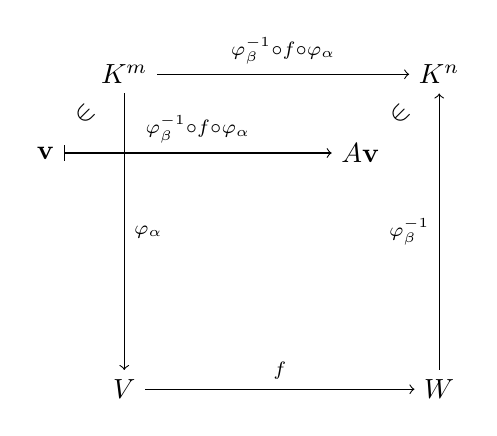
\begin{tikzpicture}[auto] 

    \node (a) at (1, 0) {$V$};
    \node (b) at (5, 0) {$W$};
    \node (c) at (1, 4) {$K^m $};
    \node (d) at (5, 4) {$K^n $};
    \node (e) at (0, 3) {${\bf v} $};
    \node (f) at (4, 3) {$A{\bf v} $};
    \node (g) at (0.5, 3.5) {\rotatebox{45}{$\in $} };
    \node (h) at (4.5, 3.5) {\rotatebox{45}{$\in $} };
    
    \draw [->] (c) to node {$\scriptstyle \varphi_{\beta}^{-1} \circ f\circ \varphi_{\alpha} $} (d);
    \draw [|->] (e) to node {$\scriptstyle \varphi_{\beta}^{-1} \circ f\circ \varphi_{\alpha} $} (f);
    \draw [->] (c) to node {$\scriptstyle \varphi_{\alpha} $} (a);
    \draw [->] (a) to node {$\scriptstyle f$} (b);
    \draw [->] (b) to node {$\scriptstyle \varphi_{\beta}^{-1} $} (d);
    
  \end{tikzpicture} 
\end{center}
\end{thm}
\begin{dfn}
この行列$A$、即ち、線形写像$f:V \rightarrow W$が与えられたときの線形写像$\varphi_{\beta}^{- 1} \circ f \circ \varphi_{\alpha}$の行列$A$をそれらの基底たち$\alpha$、$\beta$に関するその写像$f$の表現行列といい$[ f]^{\beta}_{\alpha}$と書く。
\end{dfn}
\begin{proof}
体$K$上の$m$次元、$n$次元vector空間たち$V$、$W$の基底の1つがそれぞれ$\left\langle \mathbf{v}_{i} \right\rangle_{i \in \varLambda_{m}}$、$\left\langle \mathbf{w}_{i} \right\rangle_{i \in \varLambda_{n}}$でありこれらをそれぞれ$\alpha$、$\beta$とする。線形写像$f:V \rightarrow W$が与えられたとき、それらの基底たち$\alpha$、$\beta$に関する基底変換における線形同型写像たち$\varphi_{\alpha}:K^{m} \rightarrow V$、$\varphi_{\beta}:K^{n} \rightarrow W$は線形同型写像となるのであった。したがって、その逆写像$\varphi_{\beta}^{- 1}$も線形写像でその合成写像$\varphi_{\beta}^{- 1} \circ f \circ \varphi_{\alpha}$も線形写像となる。このとき、その写像$\varphi_{\beta}^{- 1} \circ f \circ \varphi_{\alpha}$の始集合、終集合がそれぞれ$K^{m}$、$K^{n}$であるから、定理\ref{2.1.4.7}よりこの写像$\varphi_{\beta}^{- 1} \circ f \circ \varphi_{\alpha}$に対応する行列$A$がその集合$M_{nm}(K)$に存在して、$\forall\mathbf{v} \in K^{m}$に対し、$\varphi_{\beta}^{- 1} \circ f \circ \varphi_{\alpha}\left( \mathbf{v} \right) = A\mathbf{v}$が成り立つ。
\end{proof}
\begin{thm}
\label{2.1.5.4}
体$K$上の$m$次元、$n$次元vector空間たち$V$、$W$の基底の1つがそれぞれ$\left\langle \mathbf{v}_{j} \right\rangle_{j \in \varLambda_{m}}$、$\left\langle \mathbf{w}_{i} \right\rangle_{i \in \varLambda_{n}}$であり、これらをそれぞれ$\alpha$、$\beta$とするとき、それらの基底たち$\alpha 、\beta$に関する線形写像$f:V \rightarrow W$の$[ f]^{\beta}_{\alpha} \in M_{nm}(K)$なる表現行列$[ f]^{\beta}_{\alpha}$の第$(i,j)$成分$a_{ij}$は、$\forall j \in \varLambda_{m}$に対し、次式を満たす。
\begin{align*}
f\left( \mathbf{v}_{j} \right) = \sum_{i \in \varLambda_{n}} {a_{ij}\mathbf{w}_{i}}
\end{align*}
逆に、$A_{nm} = \left( a_{ij} \right)_{(i,j) \in \varLambda_{n} \times \varLambda_{m}} \in M_{nm}(K)$なるある行列$A_{nm}$が上の式を満たすなら、その行列$A_{nm}$はそれらの基底たち$\alpha $、$\beta$に関する線形写像$f:V \rightarrow W$の表現行列となる。
\end{thm}
\begin{proof}
体$K$上の$m$次元、$n$次元vector空間たち$V$、$W$の基底の1つがそれぞれ$\left\langle \mathbf{v}_{j} \right\rangle_{j \in \varLambda_{m}}$、$\left\langle \mathbf{w}_{i} \right\rangle_{i \in \varLambda_{n}}$であり、これらをそれぞれ$\alpha$、$\beta$とする。また、vector空間たち$K^{m}$、$K^{n}$の標準直交基底をそれぞれ$\left\langle \mathbf{d}_{j} \right\rangle_{j \in \varLambda_{m}}$、$\left\langle \mathbf{e}_{i} \right\rangle_{i \in \varLambda_{n}}$とおく。\par
このとき、線形写像$f:V \rightarrow W$、それらの基底たち$\alpha$、$\beta$に関する基底変換における線形同型写像たち$\varphi_{\alpha}$、$\varphi_{\beta}$を用いて次式のように考えると、
\begin{center}
  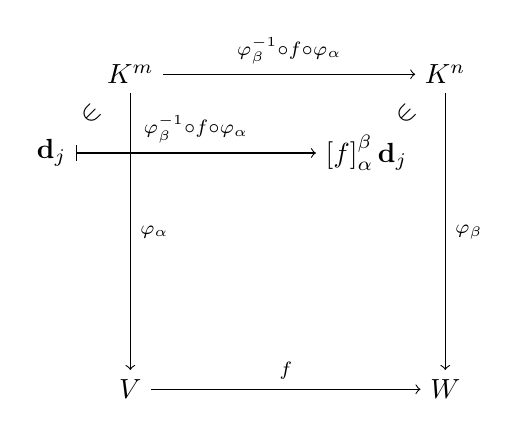
\begin{tikzpicture}[auto] 

    \node (a) at (1, 0) {$V$};
    \node (b) at (5, 0) {$W$};
    \node (c) at (1, 4) {$K^m $};
    \node (d) at (5, 4) {$K^n $};
    \node (e) at (0, 3) {${\bf d}_{j} $};
    \node (f) at (4, 3) {$\left[ f\right]^{\beta}_{\alpha} {\bf d}_{j} $};
    \node (g) at (0.5, 3.5) {\rotatebox{45}{$\in $} };
    \node (h) at (4.5, 3.5) {\rotatebox{45}{$\in $} };
    
    \draw [->] (c) to node {$\scriptstyle \varphi_{\beta}^{-1} \circ f\circ \varphi_{\alpha} $} (d);
    \draw [|->] (e) to node {$\scriptstyle \varphi_{\beta}^{-1} \circ f\circ \varphi_{\alpha} $} (f);
    \draw [->] (c) to node {$\scriptstyle \varphi_{\alpha} $} (a);
    \draw [->] (a) to node {$\scriptstyle f$} (b);
    \draw [->] (d) to node {$\scriptstyle \varphi_{\beta} $} (b);
    
    \end{tikzpicture} 
\end{center}
$\forall j \in \varLambda_{m}$に対し、次式が成り立つ。
\begin{align*}
f \circ \varphi_{\alpha}\left( \mathbf{d}_{j} \right) = f\left( \varphi_{\alpha}\left( \mathbf{d}_{j} \right) \right) = f\left( \mathbf{v}_{j} \right)
\end{align*}\par
一方で、それらの基底たち$\alpha$、$\beta$に関する線形写像$f:V \rightarrow W$の$[ f]^{\beta}_{\alpha} \in M_{nm}(K)$なる表現行列$[ f]^{\beta}_{\alpha}$が$\left( a_{ij} \right)_{(i,j) \in \varLambda_{n} \times \varLambda_{m}}$と成分表示されるとき、次のようになる。
\begin{align*}
f \circ \varphi_{\alpha}\left( \mathbf{d}_{j} \right) &= \varphi_{\beta} \circ \varphi_{\beta}^{- 1} \circ f \circ \varphi_{\alpha}\left( \mathbf{d}_{j} \right)\\
&= \varphi_{\beta}\left( \varphi_{\beta}^{- 1} \circ f \circ \varphi_{\alpha}\left( \mathbf{d}_{j} \right) \right)\\
&= \varphi_{\beta}\left( [ f]^{\beta}_{\alpha}\mathbf{d}_{j} \right)
\end{align*}
ここで、次のようになるので、
\begin{align*}
[ f]^{\beta}_{\alpha}\mathbf{d}_{j} &= \begin{pmatrix}
a_{11} & a_{12} & \cdots & a_{1j} & \cdots & a_{1m} \\
a_{21} & a_{22} & \cdots & a_{2j} & \cdots & a_{2m} \\
 \vdots & \vdots & \ddots & \vdots & \ddots & \vdots \\
a_{n1} & a_{n2} & \cdots & a_{nj} & \cdots & a_{nm} \\
\end{pmatrix}\begin{pmatrix}
0 \\
0 \\
 \vdots \\
1 \\
 \vdots \\
0 \\
\end{pmatrix} = \begin{pmatrix}
a_{1j} \\
a_{2j} \\
 \vdots \\
a_{nj} \\
\end{pmatrix}\\
&= \begin{pmatrix}
a_{1j} \\
0 \\
 \vdots \\
0 \\
\end{pmatrix} + \begin{pmatrix}
0 \\
a_{2j} \\
 \vdots \\
0 \\
\end{pmatrix} + \cdots + \begin{pmatrix}
0 \\
0 \\
 \vdots \\
a_{nj} \\
\end{pmatrix}\\
&= a_{1j}\begin{pmatrix}
1 \\
0 \\
 \vdots \\
0 \\
\end{pmatrix} + a_{2j}\begin{pmatrix}
0 \\
1 \\
 \vdots \\
0 \\
\end{pmatrix} + \cdots + a_{nj}\begin{pmatrix}
0 \\
0 \\
 \vdots \\
1 \\
\end{pmatrix}\\
&= \sum_{i \in \varLambda_{n}} {a_{ij}\mathbf{e}_{i}}
\end{align*}
したがって、次のようになる。
\begin{align*}
f \circ \varphi_{\alpha}\left( \mathbf{d}_{j} \right) &= \varphi_{\beta}\left( \sum_{i \in \varLambda_{n}} {a_{ij}\mathbf{e}_{i}} \right)\\
&= \sum_{i \in \varLambda_{n}} {a_{ij}\varphi_{\beta}\left( \mathbf{e}_{i} \right)} \\
&= \sum_{i \in \varLambda_{n}} {a_{ij}\mathbf{w}_{i}}
\end{align*}
以上より、次式が成り立つ。
\begin{align*}
f\left( \mathbf{v}_{j} \right) = f \circ \varphi_{\alpha}\left( \mathbf{d}_{j} \right) = \sum_{i \in \varLambda_{n}} {a_{ij}\mathbf{w}_{i}}
\end{align*}\par
逆に、$A_{nm} = \left( a_{ij} \right)_{(i,j) \in \varLambda_{n} \times \varLambda_{m}} \in M_{nm}(K)$なるある行列$A_{nm}$が上の式を満たすなら、$\forall j \in \varLambda_{m}$に対し、次のようになるので、
\begin{align*}
\varphi_{\beta}^{- 1} \circ f \circ \varphi_{\alpha}\left( \mathbf{d}_{j} \right) &= \varphi_{\beta}^{- 1} \circ f\left( \mathbf{v}_{j} \right)\\
&= \varphi_{\beta}^{- 1}\left( \sum_{i \in \varLambda_{n}} {a_{ij}\mathbf{w}_{i}} \right)\\
&= \sum_{i \in \varLambda_{n}} {a_{ij}\varphi_{\beta}^{- 1}\left( \mathbf{w}_{i} \right)}\\
&= \sum_{i \in \varLambda_{n}} {a_{ij}\mathbf{e}_{i}} = A_{nm}\mathbf{d}_{j}
\end{align*}
定理\ref{2.1.4.7}よりその写像$\varphi_{\beta}^{- 1} \circ f \circ \varphi_{\alpha}:K^{m} \rightarrow K^{n}$は線形写像となりその行列$A_{nm}$はそれらの基底たち$\alpha$、$\beta$に関する線形写像$f:V \rightarrow W$の表現行列となる。
\end{proof}
\begin{thm}
\label{2.1.5.5}
体$K$上の$m$次元、$n$次元vector空間たち$V$、$W$の基底の1つがそれぞれ$\left\langle \mathbf{v}_{j} \right\rangle_{j \in \varLambda_{m}}$、$\left\langle \mathbf{w}_{i} \right\rangle_{i \in \varLambda_{n}}$であり、これらをそれぞれ$\alpha$、$\beta$とし、$\forall\mathbf{v} \in V$に対し、$\mathbf{v} = \sum_{j \in \varLambda_{m}} {k_{j}\mathbf{v}_{j}}$のように書かれるとする。それらの基底たち$\alpha$、$\beta$に関する線形写像$f:V \rightarrow W$の$[ f]^{\beta}_{\alpha} \in M_{nm}(K)$なる表現行列$[ f]^{\beta}_{\alpha}$が$\left( a_{ij} \right)_{(i,j) \in \varLambda_{n} \times \varLambda_{m}}$と成分表示されるとき、次式が成り立つ。
\begin{align*}
f\left( \mathbf{v} \right) = \sum_{i \in \varLambda_{n}} {\sum_{j \in \varLambda_{m}} {a_{ij}k_{j}}\mathbf{w}_{i}}
\end{align*}
さらにいえば、そのvector$f\left( \mathbf{v} \right)$が$f\left( \mathbf{v} \right) = \sum_{i \in \varLambda_{n}} {l_{i}\mathbf{w}_{i}}$を満たすとき、次式が成り立つ。
\begin{align*}
\begin{pmatrix}
l_{1} \\
l_{2} \\
 \vdots \\
l_{n} \\
\end{pmatrix} = \begin{pmatrix}
a_{11} & a_{12} & \cdots & a_{1m} \\
a_{21} & a_{22} & \cdots & a_{2m} \\
 \vdots & \vdots & \ddots & \vdots \\
a_{n1} & a_{n2} & \cdots & a_{nm} \\
\end{pmatrix}\begin{pmatrix}
k_{1} \\
k_{2} \\
 \vdots \\
k_{m} \\
\end{pmatrix}
\end{align*}
このことは$\mathbf{k} = \begin{pmatrix}
k_{1} \\
k_{2} \\
 \vdots \\
k_{m} \\
\end{pmatrix}$、$\mathbf{l} = \begin{pmatrix}
l_{1} \\
l_{2} \\
 \vdots \\
l_{n} \\
\end{pmatrix}$としてそれらの基底たち$\alpha$、$\beta$に関する基底変換における線形同型写像たち$\varphi_{\alpha}$、$\varphi_{\beta}$を用いて次式のようにも書かれる。
\begin{center}
  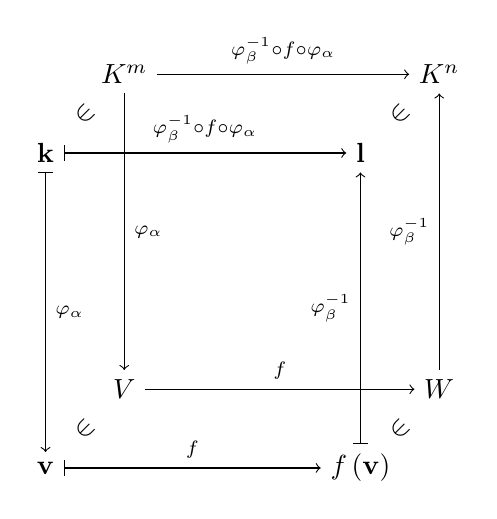
\begin{tikzpicture}[auto] 

    \node (a) at (1, 1) {$V$};
    \node (b) at (5, 1) {$W$};
    \node (c) at (1, 5) {$K^m $};
    \node (d) at (5, 5) {$K^n $};
    \node (e) at (0, 4) {${\bf k} $};
    \node (f) at (4, 4) {${\bf l} $};
    \node (g) at (0.5, 4.5) {\rotatebox{45}{$\in $} };
    \node (h) at (4.5, 4.5) {\rotatebox{45}{$\in $} };
    \node (i) at (0, 0) {${\bf v} $};
    \node (j) at (4, 0) {$f\left( {\bf v} \right) $};
    \node (k) at (0.5, 0.5) {\rotatebox{45}{$\in $} };
    \node (l) at (4.5, 0.5) {\rotatebox{45}{$\in $} };
    
    \draw [->] (c) to node {$\scriptstyle \varphi_{\beta}^{-1} \circ f\circ \varphi_{\alpha} $} (d);
    \draw [|->] (e) to node {$\scriptstyle \varphi_{\beta}^{-1} \circ f\circ \varphi_{\alpha} $} (f);
    \draw [->] (c) to node {$\scriptstyle \varphi_{\alpha} $} (a);
    \draw [|->] (e) to node {$\scriptstyle \varphi_{\alpha} $} (i);
    \draw [->] (a) to node {$\scriptstyle f$} (b);
    \draw [|->] (i) to node {$\scriptstyle f$} (j);
    \draw [->] (b) to node {$\scriptstyle \varphi_{\beta}^{-1} $} (d);
    \draw [|->] (j) to node {$\scriptstyle \varphi_{\beta}^{-1} $} (f);
    
  \end{tikzpicture} 
\end{center}
\end{thm}
\begin{proof}
体$K$上の$m$次元、$n$次元vector空間たち$V$、$W$の基底の1つがそれぞれ$\left\langle \mathbf{v}_{j} \right\rangle_{j \in \varLambda_{m}}$、$\left\langle \mathbf{w}_{i} \right\rangle_{i \in \varLambda_{n}}$であり、これらをそれぞれ$\alpha$、$\beta$とし、$\forall\mathbf{v} \in V$に対し、次式のように書かれるとする。
\begin{align*}
\mathbf{v} = \sum_{j \in \varLambda_{m}} {k_{j}\mathbf{v}_{j}}
\end{align*}
それらの基底たち$\alpha$、$\beta$に関する線形写像$f:V \rightarrow W$の$[ f]^{\beta}_{\alpha} \in M_{nm}(K)$なる表現行列$[ f]^{\beta}_{\alpha}$が$\left( a_{ij} \right)_{(i,j) \in \varLambda_{n} \times \varLambda_{m}}$と成分表示されるとき、定理\ref{2.1.5.4}より次のようになる。
\begin{align*}
f\left( \mathbf{v} \right) &= f\left( \sum_{j \in \varLambda_{m}} {k_{j}\mathbf{v}_{j}} \right)\\
&= \sum_{j \in \varLambda_{m}} {k_{j}f\left( \mathbf{v}_{j} \right)}\\
&= \sum_{j \in \varLambda_{m}} {k_{j}\sum_{i \in \varLambda_{n}} {a_{ij}\mathbf{w}_{i}}}\\
&= \sum_{j \in \varLambda_{m}} {\sum_{i \in \varLambda_{n}} {a_{ij}k_{j}\mathbf{w}_{i}}}\\
&= \sum_{i \in \varLambda_{n}} {\sum_{j \in \varLambda_{m}} {a_{ij}k_{j}}\mathbf{w}_{i}}
\end{align*}\par
さらにいえば、そのvector$f\left( \mathbf{v} \right)$が$f\left( \mathbf{v} \right) = \sum_{i \in \varLambda_{n}} {l_{i}\mathbf{w}_{i}}$を満たすとき、次のようになる。
\begin{align*}
\mathbf{0} &= \sum_{i \in \varLambda_{n}} {l_{i}\mathbf{w}_{i}} - \sum_{i \in \varLambda_{n}} {\sum_{j \in \varLambda_{m}} {a_{ij}k_{j}}\mathbf{w}_{i}}\\
&= \sum_{i \in \varLambda_{n}} {\left( l_{i} - \sum_{j \in \varLambda_{m}} {a_{ij}k_{j}} \right)\mathbf{w}_{i}}
\end{align*}
ここで、その組$\left\langle \mathbf{w}_{i} \right\rangle_{i \in \varLambda_{n}}$は基底であるから、次のようになる。
\begin{align*}
\forall i \in \varLambda_{n}\left[ l_{i} - \sum_{j \in \varLambda_{m}} {a_{ij}k_{j}} = 0 \right] &\Leftrightarrow \forall i \in \varLambda_{n}\left[ l_{i} = \sum_{j \in \varLambda_{m}} {a_{ij}k_{j}} \right]\\
&\Leftrightarrow \begin{pmatrix}
l_{1} \\
l_{2} \\
 \vdots \\
l_{n} \\
\end{pmatrix} = \begin{pmatrix}
a_{11}k_{1} + a_{12}k_{2} + \cdots + a_{1m}k_{m} \\
a_{21}k_{1} + a_{22}k_{2} + \cdots + a_{2m}k_{m} \\
 \vdots \\
a_{n1}k_{1} + a_{n2}k_{2} + \cdots + a_{nm}k_{m} \\
\end{pmatrix}\\
&\Leftrightarrow \begin{pmatrix}
l_{1} \\
l_{2} \\
 \vdots \\
l_{n} \\
\end{pmatrix} = \begin{pmatrix}
a_{11} & a_{12} & \cdots & a_{1m} \\
a_{21} & a_{22} & \cdots & a_{2m} \\
 \vdots & \vdots & \ddots & \vdots \\
a_{n1} & a_{n2} & \cdots & a_{nm} \\
\end{pmatrix}\begin{pmatrix}
k_{1} \\
k_{2} \\
 \vdots \\
k_{m} \\
\end{pmatrix}
\end{align*}
\end{proof}
\begin{thm}
\label{2.1.5.6}
体$K$上のvector空間たち$V$、$W$、線形写像たち$f:V \rightarrow W$、$g:V \rightarrow W$が与えられたとき、$\forall k,l \in K$に対し、その写像$kf + lg:V \rightarrow W$も線形写像であった。これらのvector空間たち$V$、$W$の基底の1つがそれぞれ$\alpha$、$\beta$としそれらの基底たち$\alpha$、$\beta$に関するそれらの線形写像たち$f:V \rightarrow W$、$g:V \rightarrow W$、$kf + lg:V \rightarrow W$の表現行列をそれぞれ$[ f]^{\beta}_{\alpha}$、$[ g]^{\beta}_{\alpha}$、$[ kf + lg]^{\beta}_{\alpha}$とおくと、$[ kf + lg]^{\beta}_{\alpha} = k[ f]^{\beta}_{\alpha} + l[ g]^{\beta}_{\alpha}$が成り立つ。
\end{thm}
\begin{proof}
体$K$上のvector空間たち$V$、$W$、線形写像たち$f:V \rightarrow W$、$g:V \rightarrow W$が与えられたとき、$\forall k,l \in K$に対し、その写像$kf + lg:V \rightarrow W$も線形写像であった。これらのvector空間たち$V$、$W$の基底の1つがそれぞれ$\alpha$、$\beta$としそれらの基底たち$\alpha$、$\beta$に関するそれらの線形写像たち$f:V \rightarrow W$、$g:V \rightarrow W$、$kf + lg:V \rightarrow W$の表現行列をそれぞれ$[ f]^{\beta}_{\alpha}$、$[ g]^{\beta}_{\alpha}$、$[ kf + lg]^{\beta}_{\alpha}$とおき、これらの表現行列たち$[ f]^{\beta}_{\alpha}$、$[ g]^{\beta}_{\alpha}$がそれぞれ$\left( a_{ij} \right)_{(i,j) \in \varLambda_{n} \times \varLambda_{m}}$、$\left( b_{ij} \right)_{(i,j) \in \varLambda_{n} \times \varLambda_{m}}$と成分表示されるとき、定理\ref{2.1.5.4}より$\forall j \in \varLambda_{m}$に対し、次式が成り立つ。
\begin{align*}
f\left( \mathbf{v}_{j} \right) = \sum_{i \in \varLambda_{n}} {a_{ij}\mathbf{w}_{i}},\ \ g\left( \mathbf{v}_{j} \right) = \sum_{i \in \varLambda_{n}} {b_{ij}\mathbf{w}_{i}}
\end{align*}
したがって、次のようになる。
\begin{align*}
\left( kf + lg \right)\left( \mathbf{v}_{j} \right) &= kf\left( \mathbf{v}_{j} \right) + lg\left( \mathbf{v}_{j} \right)\\
&= k\sum_{i \in \varLambda_{n}} {a_{ij}\mathbf{w}_{i}} + l\sum_{i \in \varLambda_{n}} {b_{ij}\mathbf{w}_{i}}\\
&= k\sum_{i \in \varLambda_{n}} {a_{ij}\mathbf{w}_{i}} + l\sum_{i \in \varLambda_{n}} {b_{ij}\mathbf{w}_{i}}\\
&= \sum_{i \in \varLambda_{n}} {\left( ka_{ij} + lb_{ij} \right)\mathbf{w}_{i}}
\end{align*}
このとき、定理\ref{2.1.5.4}よりそれらの基底たち$\alpha$、$\beta$に関する線形写像$kf + lg$の表現行列$[ kf + lg]^{\beta}_{\alpha}$は$\left( ka_{ij} + lb_{ij} \right)_{(i,j) \in \varLambda_{n} \times \varLambda_{m}}$のように成分表示され、したがって、次のようになる。
\begin{align*}
\left[ kf + lg \right]^{\beta}_{\alpha} &= \left( ka_{ij} + lb_{ij} \right)_{(i,j) \in \varLambda_{n} \times \varLambda_{m}}\\
&= k\left( a_{ij} \right)_{(i,j) \in \varLambda_{n} \times \varLambda_{m}} + l\left( b_{ij} \right)_{(i,j) \in \varLambda_{n} \times \varLambda_{m}}\\
&= k[ f]^{\beta}_{\alpha} + l[ g]^{\beta}_{\alpha}
\end{align*}
\end{proof}
\begin{thm}
\label{2.1.5.7}
体$K$上のvector空間たち$U$、$V$、$W$の基底の1つがそれぞれ$\alpha$、$\beta$、$\gamma$としそれらの基底たち$\alpha$、$\beta$に関する線形写像$f:U \rightarrow V$、それらの基底たち$\beta$、$\gamma$に関する線形写像$g:V \rightarrow W$、それらの基底たち$\alpha$、$\gamma$に関する線形写像$g \circ f:U \rightarrow W$の表現行列をそれぞれ$[ f]^{\beta}_{\alpha}$、$[ g]^{\gamma}_{\beta}$、$[ g \circ f]^{\gamma}_{\alpha}$とおくと、$[ g \circ f]^{\gamma}_{\alpha} = [ g]^{\gamma}_{\beta}[ f]^{\beta}_{\alpha}$が成り立つ。
\end{thm}
\begin{proof}
体$K$上の$m$次元、$n$次元、$o$次元vector空間たち$U$、$V$、$W$の基底の1つがそれぞれ$\alpha$、$\beta$、$\gamma$としそれらの基底たち$\alpha$、$\beta$に関する線形写像$f:U \rightarrow V$、それらの基底たち$\beta$、$\gamma$に関する線形写像$g:V \rightarrow W$、それらの基底たち$\alpha$、$\gamma$に関する線形写像$g \circ f:U \rightarrow W$の表現行列をそれぞれ$[ f]^{\beta}_{\alpha}$、$[ g]^{\gamma}_{\beta}$、$[ g \circ f]^{\gamma}_{\alpha}$とおくと、それらの基底たち$\alpha$、$\beta$、$\gamma$に関する基底変換における線形同型写像たち$\varphi_{\alpha}$、$\varphi_{\beta}$、$\varphi_{\gamma}$を用いて次式が成り立つ。
\begin{align*}
\varphi_{\gamma}^{- 1} \circ (g \circ f) \circ \varphi_{\alpha} &= \varphi_{\gamma}^{- 1} \circ g \circ \varphi_{\beta} \circ \varphi_{\beta}^{- 1} \circ f \circ \varphi_{\alpha}\\
&= \left( \varphi_{\gamma}^{- 1} \circ g \circ \varphi_{\beta} \right) \circ \left( \varphi_{\beta}^{- 1} \circ f \circ \varphi_{\alpha} \right)
\end{align*}
これは次のようになることを意味する。
\begin{center}
  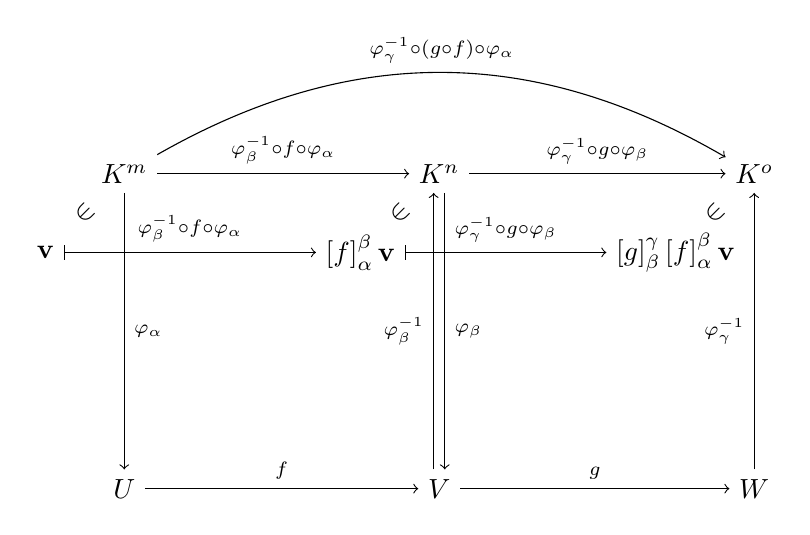
\begin{tikzpicture}[auto] 

    \node (a) at (1, 0) {$U$};
    \node (b) at (5, 0) {$V$};
    \node (c) at (1, 4) {$K^m $};
    \node (d) at (5, 4) {$K^n $};
    \node (e) at (0, 3) {${\bf v} $};
    \node (f) at (4, 3) {$\left[ f\right]^{\beta}_{\alpha} {\bf v} $};
    \node (g) at (0.5, 3.5) {\rotatebox{45}{$\in $} };
    \node (h) at (4.5, 3.5) {\rotatebox{45}{$\in $} };
    \node (i) at (9, 0) {$W$};
    \node (j) at (9, 4) {$K^o $};
    \node (k) at (8, 3) {$\left[ g\right]^{\gamma}_{\beta} \left[ f\right]^{\beta}_{\alpha} {\bf v} $};
    \node (l) at (8.5, 3.5) {\rotatebox{45}{$\in $} };
    
    \draw [->] (c) to node {$\scriptstyle \varphi_{\beta}^{-1} \circ f\circ \varphi_{\alpha} $} (d);
    \draw [|->] (e) to node {$\scriptstyle \varphi_{\beta}^{-1} \circ f\circ \varphi_{\alpha} $} (f);
    \draw [->] (c) to node {$\scriptstyle \varphi_{\alpha} $} (a);
    \draw [->] (a) to node {$\scriptstyle f$} (b);
    \draw [->, transform canvas={xshift=-2pt, yshift=0pt}] (b) to node {$\scriptstyle \varphi_{\beta}^{-1} $} (d);
    \draw [->] (d) to node {$\scriptstyle \varphi_{\gamma}^{-1} \circ g\circ \varphi_{\beta} $} (j);
    \draw [|->] (f) to node {$\scriptstyle \varphi_{\gamma}^{-1} \circ g\circ \varphi_{\beta} $} (k);
    \draw [->, transform canvas={xshift=2pt, yshift=0pt}] (d) to node {$\scriptstyle \varphi_{\beta} $} (b);
    \draw [->] (b) to node {$\scriptstyle g$} (i);
    \draw [->] (i) to node {$\scriptstyle \varphi_{\gamma}^{-1} $} (j);
    \draw [->] (c) to[bend left=30] node {$\scriptstyle \varphi_{\gamma}^{-1} \circ \left( g\circ f\right) \circ \varphi_{\alpha} $} (j);
    
    \end{tikzpicture} 
\end{center}
したがって、定義よりそれらの写像たち$\varphi_{\gamma}^{- 1} \circ g \circ \varphi_{\beta}$、$\varphi_{\beta}^{- 1} \circ f \circ \varphi_{\alpha}$の対応する行列がそれぞれ$[ f]^{\beta}_{\alpha}$、$[ g]^{\gamma}_{\beta}$と与えられることに注意すれば、その写像$\left( \varphi_{\gamma}^{- 1} \circ g \circ \varphi_{\beta} \right) \circ \left( \varphi_{\beta}^{- 1} \circ f \circ \varphi_{\alpha} \right)$の対応する行列が$[ g]^{\gamma}_{\beta}[ f]^{\beta}_{\alpha}$と与えられ、定義よりしたがって$[ g \circ f]^{\gamma}_{\alpha} = [ g]^{\gamma}_{\beta}[ f]^{\beta}_{\alpha}$が成り立つ。
\end{proof}
\begin{thm}
\label{2.1.5.8}
体$K$上の$m$次元、$n$次元vector空間たち$V$、$W$の基底の1つがそれぞれ$\alpha$、$\beta$とするとき、それらの基底たち$\alpha$、$\beta$に関する線形写像$f:V \rightarrow W$の表現行列$[ f]^{\beta}_{\alpha}$の階数${\mathrm{rank}}[ f]^{\beta}_{\alpha}$はそれらの基底たち$\alpha 、\beta$によらずその線形写像$f$の階数に等しい、即ち、${\mathrm{rank}}[ f]^{\beta}_{\alpha} = {\mathrm{rank}}f$が成り立つ。
\end{thm}
\begin{proof}
体$K$上の$m$次元、$n$次元vector空間たち$V$、$W$の基底の1つがそれぞれ$\alpha$、$\beta$とするとき、それらの基底たち$\alpha$、$\beta$に関する線形写像$f:V \rightarrow W$の表現行列$[ f]^{\beta}_{\alpha}$の階数${\mathrm{rank}}[ f]^{\beta}_{\alpha}$について考えよう。このとき、それらの基底たち$\alpha$、$\beta$に関する基底変換における線形同型写像たち$\varphi_{\alpha}$、$\varphi_{\beta}$を用いてその合成写像$\varphi_{\beta}^{- 1} \circ f \circ \varphi_{\alpha}$を$L_{[ f]^{\beta}_{\alpha}}$とおくと、次のようになり、
\begin{align*}
f &= I_{W} \circ f \circ I_{V}\\
&= \varphi_{\beta} \circ \varphi_{\beta}^{- 1} \circ f \circ \varphi_{\alpha} \circ \varphi_{\alpha}^{- 1}\\
&= \varphi_{\beta} \circ L_{[ f]^{\beta}_{\alpha}} \circ \varphi_{\alpha}^{- 1}
\end{align*}
定理\ref{2.1.2.16}より次式が成り立つ。
\begin{align*}
{\mathrm{rank}}{\varphi_{\beta}^{- 1} \circ f \circ \varphi_{\alpha}} &\leq {\mathrm{rank}}{f \circ \varphi_{\alpha}}\\
&\leq {\mathrm{rank}}f\\
&= {\mathrm{rank}}{\varphi_{\beta} \circ L_{[ f]^{\beta}_{\alpha}} \circ \varphi_{\alpha}^{- 1}}\\
&\leq {\mathrm{rank}}{L_{[ f]^{\beta}_{\alpha}} \circ \varphi_{\alpha}^{- 1}}\\
&\leq {\mathrm{rank}}L_{[ f]^{\beta}_{\alpha}}\\
&= {\mathrm{rank}}{\varphi_{\beta}^{- 1} \circ f \circ \varphi_{\alpha}}
\end{align*}
以上より${\mathrm{rank}}{\varphi_{\beta}^{- 1} \circ f \circ \varphi_{\alpha}} = {\mathrm{rank}}f$が成り立つ。ここで、定理\ref{2.1.4.12}より${\mathrm{rank}}L_{[ f]^{\beta}_{\alpha}} = {\mathrm{rank}}[ f]^{\beta}_{\alpha}$が成り立つので、その表現行列$[ f]^{\beta}_{\alpha}$の階数${\mathrm{rank}}[ f]^{\beta}_{\alpha}$はそれらの基底たち$\alpha$、$\beta$によらずその線形写像の階数${\mathrm{rank}}f$に等しい。
\end{proof}
%\hypertarget{ux57faux5e95ux5909ux63dbux884cux5217}{%
\subsubsection{基底変換行列}%\label{ux57faux5e95ux5909ux63dbux884cux5217}}
\begin{thm}
\label{2.1.5.9}
体$K$上の$n$次元vector空間$V$の2つの基底たち$\left\langle \mathbf{v}_{i} \right\rangle_{i \in \varLambda_{n}}$、$\left\langle \mathbf{w}_{i} \right\rangle_{i \in \varLambda_{n}}$が与えられこれらをそれぞれ$\alpha$、$\beta$とおく。このとき、それらの基底たち$\alpha$、$\beta$に関する基底変換における線形同型写像たち$\varphi_{\alpha}$、$\varphi_{\beta}$の合成写像$\varphi_{\beta}^{- 1} \circ \varphi_{\alpha}$に対応する$A \in M_{nn}(K)$なる行列$A$はそれらの基底たち$\alpha$、$\beta$に関する恒等写像$I_{V}:V \rightarrow V$の表現行列$\left[ I_{V} \right]^{\beta}_{\alpha}$に等しい、即ち、$A = \left[ I_{V} \right]^{\beta}_{\alpha}$が成り立つ。
\end{thm}
\begin{dfn}
このような行列$\left[ I_{V} \right]^{\beta}_{\alpha}$、即ち、線形写像$\varphi_{\beta}^{- 1} \circ \varphi_{\alpha}$の行列$\left[ I_{V} \right]^{\beta}_{\alpha}$をその基底$\alpha$からその基底$\beta$への基底変換行列という。
\end{dfn}
\begin{proof}
体$K$上の$n$次元vector空間$V$の2つの基底たち$\left\langle \mathbf{v}_{i} \right\rangle_{i \in \varLambda_{n}}$、$\left\langle \mathbf{w}_{i} \right\rangle_{i \in \varLambda_{n}}$が与えられこれらをそれぞれ$\alpha$、$\beta$とおく。このとき、次式のようにそれらの基底たち$\alpha$、$\beta$に関する基底変換における線形同型写像たち$\varphi_{\alpha}$、$\varphi_{\beta}$、恒等写像$I_{V}:V \rightarrow V$を用いて考えると、
\begin{center}
  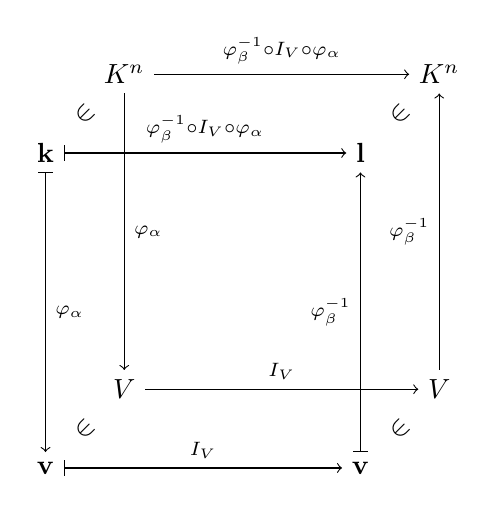
\begin{tikzpicture}[auto]

    \node (a) at (1, 1) {$V$};
    \node (b) at (5, 1) {$V$};
    \node (c) at (1, 5) {$K^n $};
    \node (d) at (5, 5) {$K^n $};
    \node (e) at (0, 4) {${\bf k} $};
    \node (f) at (4, 4) {${\bf l} $};
    \node (g) at (0.5, 4.5) {\rotatebox{45}{$\in $} };
    \node (h) at (4.5, 4.5) {\rotatebox{45}{$\in $} };
    \node (i) at (0, 0) {${\bf v} $};
    \node (j) at (4, 0) {${\bf v} $};
    \node (k) at (0.5, 0.5) {\rotatebox{45}{$\in $} };
    \node (l) at (4.5, 0.5) {\rotatebox{45}{$\in $} };
    
    \draw [->] (c) to node {$\scriptstyle \varphi_{\beta}^{-1} \circ I_V \circ \varphi_{\alpha} $} (d);
    \draw [|->] (e) to node {$\scriptstyle \varphi_{\beta}^{-1} \circ I_V \circ \varphi_{\alpha} $} (f);
    \draw [->] (c) to node {$\scriptstyle \varphi_{\alpha} $} (a);
    \draw [|->] (e) to node {$\scriptstyle \varphi_{\alpha} $} (i);
    \draw [->] (a) to node {$\scriptstyle I_V $} (b);
    \draw [|->] (i) to node {$\scriptstyle I_V $} (j);
    \draw [->] (b) to node {$\scriptstyle \varphi_{\beta}^{-1} $} (d);
    \draw [|->] (j) to node {$\scriptstyle \varphi_{\beta}^{-1} $} (f);
   
  \end{tikzpicture}
\end{center}
$\varphi_{\beta}^{- 1} \circ \varphi_{\alpha} = \varphi_{\beta}^{- 1} \circ I_{V} \circ \varphi_{\alpha}$が成り立つので、定義より明らかにその合成写像$\varphi_{\beta}^{- 1} \circ \varphi_{\alpha}$に対応する$A \in M_{nn}(K)$なる行列$A$はそれらの基底たち$\alpha$、$\beta$に関するその恒等写像$I_{V}:V \rightarrow V$の表現行列$\left[ I_{V} \right]^{\beta}_{\alpha}$に等しい。
\end{proof}
\begin{thm}
\label{2.1.5.10}
体$K$上の$n$次元vector空間$V$の2つの基底たち$\left\langle \mathbf{v}_{i} \right\rangle_{i \in \varLambda_{n}}$、$\left\langle \mathbf{w}_{i} \right\rangle_{i \in \varLambda_{n}}$が与えられこれらをそれぞれ$\alpha$、$\beta$とおく。このとき、その基底$\alpha$からその基底$\beta$への基底変換行列$\left[ I_{V} \right]^{\beta}_{\alpha}$は$\left[ I_{V} \right]^{\beta}_{\alpha} \in {\mathrm{GL}}_{n}(K)$を満たし$\left[ I_{V} \right]^{\alpha}_{\beta} = {\left[ I_{V} \right]^{\beta}_{\alpha}}^{- 1}$が成り立つ。\par
このことはそれらの基底たち$\alpha$、$\beta$に関する基底変換における線形同型写像たち$\varphi_{\alpha}$、$\varphi_{\beta}$を用いて次式のようにも書かれる。
\begin{center}
  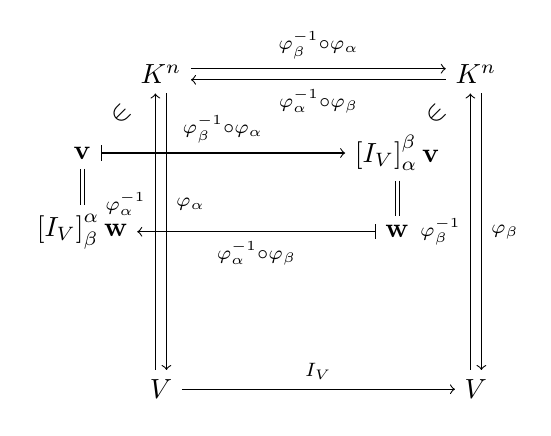
\begin{tikzpicture}[auto]

    \node (a) at (1, 0) {$V$};
    \node (b) at (5, 0) {$V$};
    \node (c) at (1, 4) {$K^n $};
    \node (d) at (5, 4) {$K^n $};
    \node (e) at (0, 3) {${\bf v} $};
    \node (f) at (4, 3) {$\left[ I_V\right]^{\beta}_{\alpha} {\bf v} $};
    \node (i) at (0, 2) {$\left[ I_V\right]^{\alpha}_{\beta} {\bf w} $};
    \node (j) at (4, 2) {${\bf w} $};
    \node (g) at (0.5, 3.5) {\rotatebox{45}{$\in $} };
    \node (h) at (4.5, 3.5) {\rotatebox{45}{$\in $} };
    
    \draw [->, transform canvas={xshift=0pt, yshift=2pt}] (c) to node {$\scriptstyle \varphi_{\beta}^{-1} \circ \varphi_{\alpha} $} (d);
    \draw [->, transform canvas={xshift=0pt, yshift=-2pt}] (d) to node {$\scriptstyle \varphi_{\alpha}^{-1} \circ \varphi_{\beta} $} (c);
    \draw [->, transform canvas={xshift=2pt, yshift=0pt}] (c) to node[xshift=0pt, yshift=10pt] {$\scriptstyle \varphi_{\alpha} $} (a);
    \draw [->, transform canvas={xshift=-2pt, yshift=0pt}] (a) to node[xshift=0pt, yshift=10pt] {$\scriptstyle \varphi_{\alpha}^{-1} $} (c);
    \draw [->] (a) to node {$\scriptstyle I_V $} (b);
    \draw [->, transform canvas={xshift=2pt, yshift=0pt}] (d) to node {$\scriptstyle \varphi_{\beta} $} (b);
    \draw [->, transform canvas={xshift=-2pt, yshift=0pt}] (b) to node {$\scriptstyle \varphi_{\beta}^{-1} $} (d);
    \draw [|->] (e) to node {$\scriptstyle \varphi_{\beta}^{-1} \circ \varphi_{\alpha} $} (f);
    \draw [|->] (j) to node {$\scriptstyle \varphi_{\alpha}^{-1} \circ \varphi_{\beta} $} (i);
    \draw [double distance=1pt] (e) to node {$\scriptstyle $} (i);
    \draw [double distance=1pt] (f) to node {$\scriptstyle $} (j);
    
    \end{tikzpicture}
\end{center}
\end{thm}
\begin{proof}
体$K$上の$n$次元vector空間$V$の2つの基底たち$\left\langle \mathbf{v}_{i} \right\rangle_{i \in \varLambda_{n}}$、$\left\langle \mathbf{w}_{i} \right\rangle_{i \in \varLambda_{n}}$が与えられこれらをそれぞれ$\alpha$、$\beta$とおく。このとき、それらの基底たち$\alpha$、$\beta$に関する基底変換における線形同型写像たち$\varphi_{\alpha}$、$\varphi_{\beta}$を用いてその基底$\alpha$からその基底$\beta$への基底変換行列$\left[ I_{V} \right]^{\beta}_{\alpha}$は定理\ref{2.1.5.9}よりその合成写像$\varphi_{\beta}^{- 1} \circ \varphi_{\alpha}$の対応する行列でもあり、それらの2つの写像たち$\varphi_{\alpha}$、$\varphi_{\beta}$は線形同型写像であったので、その合成写像$\varphi_{\beta}^{- 1} \circ \varphi_{\alpha}$も線形同型写像となる。このとき、定理\ref{2.1.4.14}よりその合成写像$\varphi_{\beta}^{- 1} \circ \varphi_{\alpha}$に対応する行列でもあるその基底$\alpha$からその基底$\beta$への基底変換行列$\left[ I_{V} \right]^{\beta}_{\alpha}$は正則行列で$\left[ I_{V} \right]^{\beta}_{\alpha} \in {\mathrm{GL}}_{n}(K)$を満たす。したがって、逆行列${\left[ I_{V} \right]^{\beta}_{\alpha}}^{- 1}$が存在しこれが対応する行列となるその写像はその写像$\varphi_{\beta}^{- 1} \circ \varphi_{\alpha}$の逆写像となる。このとき、次のようになるので、
\begin{align*}
I_{K^{n}} &= \varphi_{\alpha}^{- 1} \circ \varphi_{\alpha}\\
&= \varphi_{\alpha}^{- 1} \circ \left( \varphi_{\beta} \circ \varphi_{\beta}^{- 1} \right) \circ \varphi_{\alpha}\\
&= \left( \varphi_{\alpha}^{- 1} \circ \varphi_{\beta} \right) \circ \left( \varphi_{\beta}^{- 1} \circ \varphi_{\alpha} \right)\\
I_{K^{n}} &= \varphi_{\alpha} \circ \varphi_{\alpha}^{- 1}\\
&= \varphi_{\alpha} \circ \left( \varphi_{\beta}^{- 1} \circ \varphi_{\beta} \right) \circ \varphi_{\alpha}^{- 1}\\
&= \left( \varphi_{\alpha} \circ \varphi_{\beta}^{- 1} \right) \circ \left( \varphi_{\beta} \circ \varphi_{\alpha}^{- 1} \right)
\end{align*}
その合成写像$\varphi_{\alpha} \circ \varphi_{\beta}^{- 1}$は対応する行列が${\left[ I_{V} \right]^{\beta}_{\alpha}}^{- 1}$となるようなその合成写像$\varphi_{\beta}^{- 1} \circ \varphi_{\alpha}$の逆写像となりこれに対応する行列が上記の定理より$\left[ I_{V} \right]^{\alpha}_{\beta}$となるので、$\left[ I_{V} \right]^{\alpha}_{\beta} = {\left[ I_{V} \right]^{\beta}_{\alpha}}^{- 1}$が成り立つ。
\end{proof}\par
以上の議論により体$K$上の$n$次元vector空間$V$の2つの基底たち$\left\langle \mathbf{v}_{i} \right\rangle_{i \in \varLambda_{n}}$、$\left\langle \mathbf{w}_{i} \right\rangle_{i \in \varLambda_{n}}$が与えられこれらをそれぞれ$\alpha$、$\beta$とおく。$\forall\mathbf{v} \in V$に対し、次式のように書かれるとする。
\begin{align*}
\mathbf{v} = \sum_{i \in \varLambda_{n}} {k_{i}\mathbf{v}_{i}} = \sum_{i \in \varLambda_{n}} {l_{i}\mathbf{w}_{i}}
\end{align*}
その基底$\alpha$からその基底$\beta$への基底変換行列$\left[ I_{V} \right]^{\beta}_{\alpha}$が$\left( a_{ij} \right)_{(i,j) \in \varLambda_{n} \times \varLambda_{n}}$と成分表示されるとき、$\forall j \in \varLambda_{n}$に対し、次式が成り立つ。
\begin{align*}
\mathbf{v}_{j} = \sum_{i \in \varLambda_{n}} {a_{ij}\mathbf{w}_{i}}
\end{align*}
逆に、$A_{nn} = \left( a_{ij} \right)_{(i,j) \in \varLambda_{n} \times \varLambda_{n}} \in M_{nn}(K)$なるある行列$A_{nn}$が上の式を満たすなら、その行列$A_{nn}$はその基底$\alpha$からその基底$\beta$への基底変換行列となる。さらにいえば、次式が成り立つ。
\begin{align*}
\begin{pmatrix}
l_{1} \\
l_{2} \\
 \vdots \\
l_{n} \\
\end{pmatrix} = \begin{pmatrix}
a_{11} & a_{12} & \cdots & a_{1n} \\
a_{21} & a_{22} & \cdots & a_{2n} \\
 \vdots & \vdots & \ddots & \vdots \\
a_{n1} & a_{n2} & \cdots & a_{nn} \\
\end{pmatrix}\begin{pmatrix}
k_{1} \\
k_{2} \\
 \vdots \\
k_{n} \\
\end{pmatrix}
\end{align*}
このことは$\mathbf{k} = \begin{pmatrix}
k_{1} \\
k_{2} \\
 \vdots \\
k_{n} \\
\end{pmatrix}$、$\mathbf{l} = \begin{pmatrix}
l_{1} \\
l_{2} \\
 \vdots \\
l_{n} \\
\end{pmatrix}$として次式のようにも書かれる。
\begin{center}
  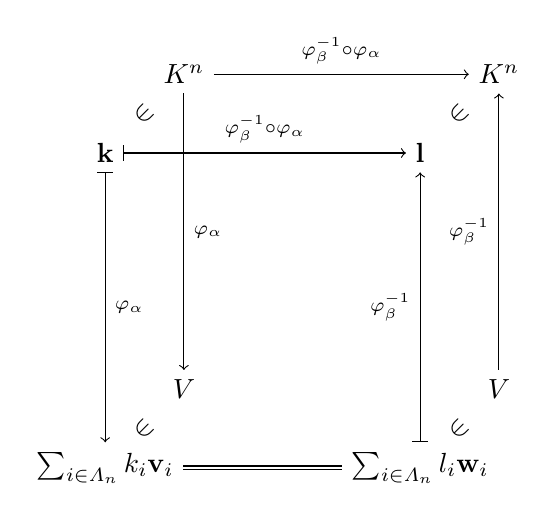
\begin{tikzpicture}[auto]

    \node (a) at (1, 1) {$V$};
    \node (b) at (5, 1) {$V$};
    \node (c) at (1, 5) {$K^n $};
    \node (d) at (5, 5) {$K^n $};
    \node (e) at (0, 4) {${\bf k} $};
    \node (f) at (4, 4) {${\bf l} $};
    \node (g) at (0.5, 4.5) {\rotatebox{45}{$\in $} };
    \node (h) at (4.5, 4.5) {\rotatebox{45}{$\in $} };
    \node (i) at (0, 0) {$\sum_{i\in \varLambda_{n} } k_i {\bf v}_i $};
    \node (j) at (4, 0) {$\sum_{i\in \varLambda_{n} } l_i {\bf w}_i $};
    \node (k) at (0.5, 0.5) {\rotatebox{45}{$\in $} };
    \node (l) at (4.5, 0.5) {\rotatebox{45}{$\in $} };
    
    \draw [->] (c) to node {$\scriptstyle \varphi_{\beta}^{-1} \circ \varphi_{\alpha} $} (d);
    \draw [|->] (e) to node {$\scriptstyle \varphi_{\beta}^{-1} \circ \varphi_{\alpha} $} (f);
    \draw [->] (c) to node {$\scriptstyle \varphi_{\alpha} $} (a);
    \draw [|->] (e) to node {$\scriptstyle \varphi_{\alpha} $} (i);
    
    
    \draw [->] (b) to node {$\scriptstyle \varphi_{\beta}^{-1} $} (d);
    \draw [|->] (j) to node {$\scriptstyle \varphi_{\beta}^{-1} $} (f);
    \draw [double distance=1pt] (i) to node {$\scriptstyle $} (j);
    
    \end{tikzpicture}
\end{center}
\begin{thm}
\label{2.1.5.11}
体$K$上の$n$次元vector空間$V$のある基底$\left\langle \mathbf{v}_{i} \right\rangle_{i \in \varLambda_{n}}$が与えられこれを$\alpha$とおく。このとき、$A \in {\mathrm{GL}}_{n}(K)$なる行列$A$がその基底$\alpha$からある基底$\beta$への基底変換行列となるようなその基底$\beta$が存在する。
\end{thm}
\begin{proof}
体$K$上の$n$次元vector空間$V$のある基底$\left\langle \mathbf{v}_{i} \right\rangle_{i \in \varLambda_{n}}$が与えられこれを$\alpha$とおく。このとき、$A \in {\mathrm{GL}}_{n}(K)$なる行列$A$がある写像$L_{A}:K^{n} \rightarrow K^{n}$に対応する行列となるようなその写像$L_{A}$の逆写像$L_{A}^{- 1}$は定理より明らかに線形同型写像でその基底$\alpha$に関する基底変換における線形同型写像$\varphi_{\alpha}$を用いて得られる合成写像$\varphi_{\alpha} \circ L_{A}^{- 1}:K^{n} \rightarrow V$は線形同型写像となり、次式のように考えれば、
\begin{center}
  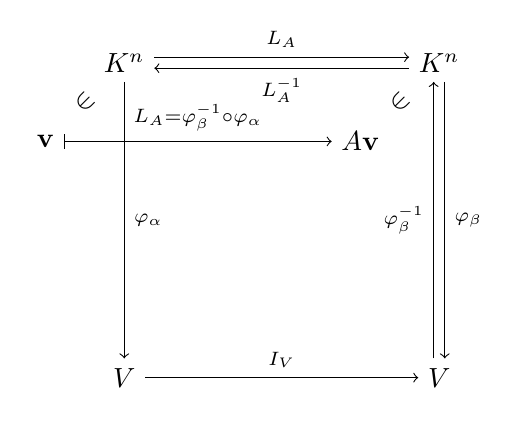
\begin{tikzpicture}[auto]

    \node (a) at (1, 1) {$V$};
    \node (b) at (5, 1) {$V$};
    \node (c) at (1, 5) {$K^n $};
    \node (d) at (5, 5) {$K^n $};
    \node (e) at (0, 4) {${\bf v} $};
    \node (f) at (4, 4) {$A{\bf v} $};
    \node (g) at (0.5, 4.5) {\rotatebox{45}{$\in $} };
    \node (h) at (4.5, 4.5) {\rotatebox{45}{$\in $} };
    
    \draw [->, transform canvas={xshift=0pt, yshift=2pt}] (c) to node {$\scriptstyle L_A $} (d);
    \draw [->, transform canvas={xshift=0pt, yshift=-2pt}] (d) to node {$\scriptstyle L_A^{-1} $} (c);
    \draw [|->] (e) to node {$\scriptstyle L_A =\varphi_{\beta}^{-1} \circ \varphi_{\alpha} $} (f);
    \draw [->] (c) to node {$\scriptstyle \varphi_{\alpha} $} (a);
    \draw [->] (a) to node {$\scriptstyle I_V $} (b);
    \draw [->, transform canvas={xshift=2pt, yshift=0pt}] (d) to node {$\scriptstyle \varphi_{\beta} $} (b);
    \draw [->, transform canvas={xshift=-2pt, yshift=0pt}] (b) to node {$\scriptstyle \varphi_{\beta}^{-1} $} (d);
    
  \end{tikzpicture} 
\end{center}
定理\ref{2.1.5.2}より、そのvector空間$K^{n}$の標準直交基底$\left\langle \mathbf{e}_{i} \right\rangle_{i \in \varLambda_{n}}$を用いたvectorsの組$\left\langle \varphi_{\alpha} \circ L_{A}^{- 1}\left( \mathbf{e}_{i} \right) \right\rangle_{i \in \varLambda_{n}}$はそのvector空間$V$の基底となり、これを$\beta$とおくと、$\varphi_{\alpha} \circ L_{A}^{- 1} = \varphi_{\beta}$が成り立つ。このとき、次のようになるので、
\begin{align*}
L_{A} &= \left( L_{A}^{- 1} \right)^{- 1}\\
&= \left( I_{K^{n}} \circ L_{A}^{- 1} \right)^{- 1}\\
&= \left( \varphi_{\alpha}^{- 1} \circ \varphi_{\alpha} \circ L_{A}^{- 1} \right)^{- 1}\\
&= \left( \varphi_{\alpha}^{- 1} \circ \varphi_{\beta} \right)^{- 1}\\
&= \varphi_{\beta}^{- 1} \circ \varphi_{\alpha}
\end{align*}
定義より明らかにその行列$A$がその基底$\alpha$からある基底$\beta$への基底変換行列となる。
\end{proof}
\begin{thm}
\label{2.1.5.12}
体$K$上の$m$次元、$n$次元vector空間たち$V$、$W$の基底の2つをそれぞれ$\alpha_{1}$、$\alpha_{2}$、$\beta_{1}$、$\beta_{2}$とするとき、それらの基底たちそれぞれ$\alpha_{1}$、$\beta_{1}$、$\alpha_{2}$、$\beta_{2}$に関する線形写像$f:V \rightarrow W$の表現行列たちそれぞれ$[ f]^{\beta_{1}}_{\alpha_{1}}$、$[ f]^{\beta_{2}}_{\alpha_{2}}$とそれらのvector空間$V$、$W$の基底変換行列たち$\left[ I_{V} \right]^{\alpha_{2}}_{\alpha_{1}}$、$\left[ I_{W} \right]^{\beta_{2}}_{\beta_{1}}$について、$\left[ I_{W} \right]^{\beta_{2}}_{\beta_{1}}[ f]^{\beta_{1}}_{\alpha_{1}} = [ f]^{\beta_{2}}_{\alpha_{2}}\left[ I_{V} \right]^{\alpha_{2}}_{\alpha_{1}}$が成り立つ。
\end{thm}
\begin{proof}
体$K$上の$m$次元、$n$次元vector空間たち$V$、$W$の基底の2つをそれぞれ$\alpha_{1}$、$\alpha_{2}$、$\beta_{1}$、$\beta_{2}$とするとき、それらの基底たちそれぞれ$\alpha_{1}$、$\beta_{1}$、$\alpha_{2}$、$\beta_{2}$に関する線形写像$f:V \rightarrow W$の表現行列たちそれぞれ$[ f]^{\beta_{1}}_{\alpha_{1}}$、$[ f]^{\beta_{2}}_{\alpha_{2}}$とそれらのvector空間$V$、$W$の基底変換行列たち$\left[ I_{V} \right]^{\alpha_{2}}_{\alpha_{1}}$、$\left[ I_{W} \right]^{\beta_{2}}_{\beta_{1}}$について、それらの基底たち$\alpha_{1}$、$\beta_{1}$、$\alpha_{2}$、$\beta_{2}$に関する基底変換における線形同型写像たち$\varphi_{\alpha_{1}}$、$\varphi_{\beta_{1}}$、$\varphi_{\alpha_{2}}$、$\varphi_{\beta_{2}}$を用いて次のようになり、
\begin{align*}
\left( \varphi_{\beta_{2}}^{- 1} \circ \varphi_{\beta_{1}} \right) \circ \left( \varphi_{\beta_{1}}^{- 1} \circ f \circ \varphi_{\alpha_{1}} \right) &= \varphi_{\beta_{2}}^{- 1} \circ \left( \varphi_{\beta_{1}} \circ \varphi_{\beta_{1}}^{- 1} \right) \circ f \circ \varphi_{\alpha_{1}}\\
&= \varphi_{\beta_{2}}^{- 1} \circ I_{W} \circ f \circ I_{V} \circ \varphi_{\alpha_{1}}\\
&= \varphi_{\beta_{2}}^{- 1} \circ f \circ \left( \varphi_{\alpha_{2}} \circ \varphi_{\alpha_{2}}^{- 1} \right) \circ \varphi_{\alpha_{1}}\\
&= \left( \varphi_{\beta_{2}}^{- 1} \circ f \circ \varphi_{\alpha_{2}} \right) \circ \left( \varphi_{\alpha_{2}}^{- 1} \circ \varphi_{\alpha_{1}} \right)
\end{align*}
次式より明らかに、
\begin{center}
  \begin{tikzpicture}[auto]

    \node (a) at (2, 6) {$K^m $};
    \node (b) at (7, 6) {$K^n $};
    \node (c) at (0, 5) {$K^m $};
    \node (d) at (5, 5) {$K^n $};
    \node (e) at (2, 1) {$V$};
    \node (f) at (7, 1) {$W$};
    \node (g) at (0, 0) {$V$};
    \node (h) at (5, 0) {$W$};
    \node (sb) at (10, 6) {$\ $};
    
    \draw [->] (a) to node {$\scriptstyle \varphi_{\beta_1 }^{-1} \circ f\circ \varphi_{\alpha_1 } $} (b);
    \draw [->] (c) to node[xshift=25pt, yshift=0pt] {$\scriptstyle \varphi_{\beta_2 }^{-1} \circ f\circ \varphi_{\alpha_2 } $} (d);
    \draw [>->>] (a) to node {$\scriptstyle \varphi_{\alpha_2 }^{-1} \circ \varphi_{\alpha_1 } $} (c);
    \draw [>->>] (b) to node {$\scriptstyle \varphi_{\beta_2 }^{-1} \circ \varphi_{\beta_1 } $} (d);
    \draw [>->>] (a) to node {$\scriptstyle \varphi_{\alpha_1 } $} (e);
    \draw [>->>] (b) to node {$\scriptstyle \varphi_{\beta_1 } $} (f);
    \draw [>->>] (c) to node {$\scriptstyle \varphi_{\alpha_2 } $} (g);
    \draw [>->>] (d) to node {$\scriptstyle \varphi_{\beta_2 } $} (h);
    \draw [->] (e) to node[xshift=-5pt, yshift=0pt] {$\scriptstyle f$} (f);
    \draw [->] (g) to node {$\scriptstyle f$} (h);
    \draw [>->>] (e) to node {$\scriptstyle I_V $} (g);
    \draw [>->>] (f) to node {$\scriptstyle I_W $} (h);
    
    \end{tikzpicture} 
    \begin{tikzpicture}[auto]
    
    \node (a) at (2, 6) {${\bf k} $};
    %\node (b) at (7, 6) {$\left[ f\right]^{\beta_1 }_{\alpha_1 } {\bf k} $};
    \node (c) at (0, 5) {$\left[ I_V\right]^{\alpha_2 }_{\alpha_1 } {\bf k} $};
    \node (d) at (5, 5) {$\left[ f\right]^{\beta_2 }_{\alpha_2 } \left[ I_V \right]^{\alpha_2 }_{\alpha_1 } {\bf k} $};
    \node (e) at (2, 1) {${\bf v} $};
    %\node (f) at (7, 1) {$f\left( {\bf v}\right) $};
    \node (g) at (0, 0) {${\bf v} $};
    \node (h) at (5, 0) {$f\left( {\bf v}\right) $};
    
    %\draw [|->] (a) to node {$\scriptstyle \varphi_{\beta_1 }^{-1} \circ f\circ \varphi_{\alpha_1 } $} (b);
    \draw [|->] (c) to node[xshift=0pt, yshift=-15pt] {$\scriptstyle \varphi_{\beta_2 }^{-1} \circ f\circ \varphi_{\alpha_2 } $} (d);
    \draw [|->] (a) to node {$\scriptstyle \varphi_{\alpha_2 }^{-1} \circ \varphi_{\alpha_1 } $} (c);
    %\draw [|->] (b) to node {$\scriptstyle \varphi_{\beta_2 }^{-1} \circ \varphi_{\beta_1 } $} (d);
    \draw [|->] (a) to node {$\scriptstyle \varphi_{\alpha_1 } $} (e);
    %\draw [|->] (b) to node {$\scriptstyle \varphi_{\beta_1 } $} (f);
    \draw [|->] (c) to node {$\scriptstyle \varphi_{\alpha_2 } $} (g);
    \draw [|->] (d) to node {$\scriptstyle \varphi_{\beta_2 } $} (h);
    %\draw [|->] (e) to node {$\scriptstyle f$} (f);
    \draw [|->] (g) to node {$\scriptstyle f$} (h);
    \draw [double distance=1pt] (e) to node {$\scriptstyle $} (g);
    %\draw [double distance=1pt] (f) to node {$\scriptstyle $} (h);
    
    %\end{tikzpicture} 
    
    %\vskip \baselineskip 
    
    %\begin{tikzpicture}[auto]
    
    \node (sa) at (5, 6) {${\bf k} $};
    \node (sb) at (10, 6) {$\left[ f\right]^{\beta_1 }_{\alpha_1 } {\bf k} $};
    %\node (sc) at (3, 5) {$\left[ I_V\right]^{\alpha_2 }_{\alpha_1 } {\bf k} $};
    \node (sd) at (8, 5) {$\left[ I_W \right]^{\beta_2 }_{\beta_1 } \left[ f\right]^{\beta_1 }_{\alpha_1 } {\bf k} $};
    \node (se) at (4.5, 1) {${\bf v} $};
    \node (sf) at (10, 1) {$f\left( {\bf v}\right) $};
    %\node (sg) at (3, 0) {${\bf v} $};
    \node (sh) at (8, 0) {$f\left( {\bf v}\right) $};
    
    \draw [|->] (sa) to node {$\scriptstyle \varphi_{\beta_1 }^{-1} \circ f\circ \varphi_{\alpha_1 } $} (sb);
    %\draw [|->] (sc) to node {$\scriptstyle \varphi_{\beta_2 }^{-1} \circ f\circ \varphi_{\alpha_2 } $} (sd);
    %\draw [|->] (sa) to node {$\scriptstyle \varphi_{\alpha_2 }^{-1} \circ \varphi_{\alpha_1 } $} (sc);
    \draw [|->] (sb) to node {$\scriptstyle \varphi_{\beta_2 }^{-1} \circ \varphi_{\beta_1 } $} (sd);
    %\draw [|->] (sa) to node {$\scriptstyle \varphi_{\alpha_1 } $} (se);
    \draw [|->] (sb) to node {$\scriptstyle \varphi_{\beta_1 } $} (sf);
    %\draw [|->] (sc) to node {$\scriptstyle \varphi_{\alpha_2 } $} (sg);
    %\draw [|->] (sd) to node {$\scriptstyle \varphi_{\beta_2 } $} (sh);
    \draw [|->] (se) to node {$\scriptstyle f$} (sf);
    %\draw [|->] (sg) to node {$\scriptstyle f$} (sh);
    %\draw [double distance=1pt] (se) to node {$\scriptstyle $} (sg);
    \draw [double distance=1pt] (sf) to node {$\scriptstyle $} (sh);
    \draw [double distance=1pt] (a) to node {$\scriptstyle $} (sa);
    \draw [double distance=1pt] (e) to node {$\scriptstyle $} (se);
    \draw [double distance=1pt] (d) to node {$\scriptstyle $} (sd);
    \draw [double distance=1pt] (h) to node {$\scriptstyle $} (sh);
    
    \end{tikzpicture} 
\end{center}
その写像$\varphi_{\beta_{2}}^{- 1} \circ \varphi_{\beta_{1}}:K^{n} \rightarrow K^{n}$に対応する行列がその基底$\beta_{1}$からその基底$\beta_{2}$へのその基底変換行列$\left[ I_{W} \right]^{\beta_{2}}_{\beta_{1}}$となるかつ、定義より明らかにその写像$\varphi_{\beta_{1}}^{- 1} \circ f \circ \varphi_{\alpha_{1}}:K^{m} \rightarrow K^{n}$に対応する行列がそれらの基底たちそれぞれ$\alpha_{1}$、$\beta_{1}$に関する線形写像$f:V \rightarrow W$の表現行列$[ f]^{\beta_{1}}_{\alpha_{1}}$となるので、その合成写像$\left( \varphi_{\beta_{2}}^{- 1} \circ \varphi_{\beta_{1}} \right) \circ \left( \varphi_{\beta_{1}}^{- 1} \circ f \circ \varphi_{\alpha_{1}} \right)$に対応する行列は$\left[ I_{W} \right]^{\beta_{2}}_{\beta_{1}}[ f]^{\beta_{1}}_{\alpha_{1}}$となる。同様にして、その合成写像$\left( \varphi_{\beta_{2}}^{- 1} \circ f \circ \varphi_{\alpha_{2}} \right) \circ \left( \varphi_{\alpha_{2}}^{- 1} \circ \varphi_{\alpha_{1}} \right)$に対応する行列は$[ f]^{\beta_{2}}_{\alpha_{2}}\left[ I_{V} \right]^{\alpha_{2}}_{\alpha_{1}}$となるので、$\left[ I_{W} \right]^{\beta_{2}}_{\beta_{1}}[ f]^{\beta_{1}}_{\alpha_{1}} = [ f]^{\beta_{2}}_{\alpha_{2}}\left[ I_{V} \right]^{\alpha_{2}}_{\alpha_{1}}$が成り立つ。
\end{proof}
\begin{thm}
\label{2.1.5.13}
体$K$上の$m$次元、$n$次元vector空間たち$V$、$W$の基底の1つがそれぞれ$\alpha$、$\beta$とするとき、それらの基底たち$\alpha 、\beta$に関する線形写像$f:V \rightarrow W$の表現行列$[ f]^{\beta}_{\alpha}$が${\mathrm{rank}}f = r$として次式のように書かれるようなそれらの基底たち$\alpha$、$\beta$が存在する。
\begin{align*}
[ f]^{\beta}_{\alpha} = \begin{pmatrix}
I_{r} & O \\
O & O \\
\end{pmatrix}
\end{align*}
\end{thm}
\begin{proof}
体$K$上の$m$次元、$n$次元vector空間たち$V$、$W$が与えられたとする。このとき、次元公式より線形写像$f:V \rightarrow W$の核$\ker f$は${\mathrm{rank}}f = r$として$m - r$次元でありこれの基底の1つを$\left\langle \mathbf{v}_{i} \right\rangle_{i \in \varLambda_{m} \setminus \varLambda_{r}}$とおきこれを拡張してそのvector空間$V$の基底を$\left\langle \mathbf{v}_{i} \right\rangle_{i \in \varLambda_{m}}$としこれを$\alpha$とおく。このとき、vectorの組$\left\langle f\left( \mathbf{v}_{i} \right) \right\rangle_{i \in \varLambda_{r}}$は定理\ref{2.1.2.13}よりその部分空間$V(f)$の基底となるのであった。そこで、これを、$\forall i \in \varLambda_{r}$に対し、$\mathbf{w}_{i} = f\left( \mathbf{v}_{i} \right)$となるように拡張したそのvector空間$W$の基底$\left\langle \mathbf{w}_{i} \right\rangle_{i \in \varLambda_{n}}$を$\beta$とおく。このとき、$\forall j \in \varLambda_{m}$に対し、$j \in \varLambda_{r}$のとき、次のようになるし、
\begin{align*}
f\left( \mathbf{v}_{j} \right) = \mathbf{w}_{j} = \sum_{i \in \varLambda_{n} \setminus \left\{ j \right\}} {0\mathbf{w}_{i}} + 1\mathbf{w}_{j} = \sum_{i \in \varLambda_{n}} {\delta_{ij}\mathbf{w}_{i}}
\end{align*}
$j \in \varLambda_{m} \setminus \varLambda_{r}$のとき、核の定義より次のようになる。
\begin{align*}
f\left( \mathbf{v}_{j} \right) = \mathbf{0} = \sum_{i \in \varLambda_{n}} {0\mathbf{w}_{i}}
\end{align*}
定理\ref{2.1.5.4}よりそれらの基底たち$\alpha 、\beta$に関する線形写像$f:V \rightarrow W$の表現行列$[ f]^{\beta}_{\alpha}$は次のようになる。
\begin{align*}
[ f]^{\beta}_{\alpha} &= \begin{pmatrix}
\delta_{11} & \delta_{12} & \cdots & \delta_{1r} & 0 & 0 & \cdots & 0 \\
\delta_{21} & \delta_{22} & \cdots & \delta_{2r} & 0 & 0 & \cdots & 0 \\
 \vdots & \vdots & \ddots & \vdots & \vdots & \vdots & \ddots & \vdots \\
\delta_{r1} & \delta_{r2} & \cdots & \delta_{rr} & 0 & 0 & \cdots & 0 \\
\delta_{r + 1,1} & \delta_{r + 1,2} & \cdots & \delta_{r + 1,r} & 0 & 0 & \cdots & 0 \\
\delta_{r + 2,1} & \delta_{r + 2,2} & \cdots & \delta_{r + 2,r} & 0 & 0 & \cdots & 0 \\
 \vdots & \vdots & \ddots & \vdots & \vdots & \vdots & \ddots & \vdots \\
\delta_{n1} & \delta_{n2} & \cdots & \delta_{nr} & 0 & 0 & \cdots & 0 \\
\end{pmatrix}\\
&= \begin{pmatrix}
1 & 0 & \cdots & 0 & 0 & 0 & \cdots & 0 \\
0 & 1 & \cdots & 0 & 0 & 0 & \cdots & 0 \\
 \vdots & \vdots & \ddots & \vdots & \vdots & \vdots & \ddots & \vdots \\
0 & 0 & \cdots & 1 & 0 & 0 & \cdots & 0 \\
0 & 0 & \cdots & 0 & 0 & 0 & \cdots & 0 \\
0 & 0 & \cdots & 0 & 0 & 0 & \cdots & 0 \\
 \vdots & \vdots & \ddots & \vdots & \vdots & \vdots & \ddots & \vdots \\
0 & 0 & \cdots & 0 & 0 & 0 & \cdots & 0 \\
\end{pmatrix}\\
&= \begin{pmatrix}
I_{r} & O \\
O & O \\
\end{pmatrix}
\end{align*}
\end{proof}
%\hypertarget{ux7ddaux5f62ux5199ux50cfux306eux884cux5217ux8868ux73fe}{%
\subsubsection{線形写像の行列表現}%\label{ux7ddaux5f62ux5199ux50cfux306eux884cux5217ux8868ux73fe}}
\begin{thm}
\label{2.1.5.14}
体$K$上の$m$次元、$n$次元vector空間たち$V$、$W$の基底の1つがそれぞれ$\left\langle \mathbf{v}_{j} \right\rangle_{j \in \varLambda_{m}}$、$\left\langle \mathbf{w}_{i} \right\rangle_{i \in \varLambda_{n}}$であり、これらをそれぞれ$\alpha$、$\beta$とすると、それらの基底たち$\alpha 、\beta$に関する線形写像$f:V \rightarrow W$の$[ f]^{\beta}_{\alpha} \in M_{nm}(K)$なる表現行列$[ f]^{\beta}_{\alpha}$を用いて次式のように定義される写像$F_{\alpha \rightarrow \beta}$はvector空間$L(V,W)$からvector空間$M_{nm}(K)$への線形同型写像である。なお、$L(V,W)$はそのvector空間$V$からそのvector空間$W$への線形写像全体の集合である。
\begin{align*}
F_{\alpha \rightarrow \beta}:L(V,W) \rightarrow M_{nm}(K);f \mapsto [ f]^{\beta}_{\alpha}
\end{align*}
\end{thm}
\begin{proof}
体$K$上の$m$次元、$n$次元vector空間たち$V$、$W$の基底の1つがそれぞれ$\left\langle \mathbf{v}_{j} \right\rangle_{j \in \varLambda_{m}}$、$\left\langle \mathbf{w}_{i} \right\rangle_{i \in \varLambda_{n}}$であり、これらをそれぞれ$\alpha$、$\beta$とする。それらの基底たち$\alpha$、$\beta$に関する線形写像$f:V \rightarrow W$の$[ f]^{\beta}_{\alpha} \in M_{nm}(K)$なる表現行列$[ f]^{\beta}_{\alpha}$を用いて次式のように定義される写像$F_{\alpha \rightarrow \beta}$を考えよう。
\begin{align*}
F_{\alpha \rightarrow \beta}:L(V,W) \rightarrow M_{nm}(K);f \mapsto [ f]^{\beta}_{\alpha}
\end{align*}\par
このとき、2つの集合たち$L(V,W)$、$M_{nm}(K)$はvector空間で、定理\ref{2.1.5.6}より$\forall f,g \in L(V,W)\forall k,l \in K$に対し、$kf + lg \in L(V,W)$が成り立ち、それらの基底たち$\alpha$、$\beta$に関する線形写像たち$f$、$g$、$kf + lg$の表現行列たち$[ f]^{\beta}_{\alpha}$、$[ g]^{\beta}_{\alpha}$、$[ kf + lg]^{\beta}_{\alpha}$が与えられたとき、次のようになるので、
\begin{align*}
F_{\alpha \rightarrow \beta}\left( kf + lg \right) &= \left[ kf + lg \right]^{\beta}_{\alpha}\\
&= k[ f]^{\beta}_{\alpha} + l[ g]^{\beta}_{\alpha}\\
&= kF_{\alpha \rightarrow \beta}(f) + lF_{\alpha \rightarrow \beta}(g)
\end{align*}
その写像$F_{\alpha \rightarrow \beta}$は線形的である。\par
また、定理\ref{2.1.5.4}より$A_{nm} = \left( a_{ij} \right)_{(i,j) \in \varLambda_{n} \times \varLambda_{m}} \in M_{nm}(K)$なるある行列$A_{nm}$が、$\forall j \in \varLambda_{m}$に対し、次式を満たすようにすれば、
\begin{align*}
f:V \rightarrow W;\mathbf{v}_{j} \mapsto \sum_{i \in \varLambda_{n}} {a_{ij}\mathbf{w}_{i}}
\end{align*}
その行列$A_{nm}$はそれらの基底たち$\alpha$、$\beta$に関する線形写像$f:V \rightarrow W$の表現行列となるので、逆写像が存在することから、その写像$F_{\alpha \rightarrow \beta}$は全単射となる。\par
以上より、その写像$F_{\alpha \rightarrow \beta}$は線形的であるかつ、全単射であるので、線形同型写像である。
\end{proof}
\begin{thm}
\label{2.1.5.15}
体$K$上の$n$次元vector空間$V$の基底の1つを$\alpha$とし、その基底$\alpha$に関する線形写像$f:V \rightarrow V$の$[ f]_{\alpha}^{\alpha} \in M_{nn}(K)$なる表現行列$[ f]_{\alpha}^{\alpha}$を用いて写像$F_{\alpha \rightarrow \alpha}$が次式のように定義されれば、
\begin{align*}
F_{\alpha \rightarrow \alpha}:L(V,W) \rightarrow M_{nn}(K);f \mapsto [ f]_{\alpha}^{\alpha}
\end{align*}
恒等写像$I_{V}:V \rightarrow V;\mathbf{v} \mapsto \mathbf{v}$について、$n$次単位行列$I_{n}$を用いて$\left[ I_{V} \right]_{\alpha}^{\alpha} = F_{\alpha \rightarrow \alpha}\left( I_{V} \right) = I_{n}$が成り立つ。
\end{thm}
\begin{proof}
体$K$上の$n$次元vector空間$V$の基底の1つを$\alpha$とし、その基底$\alpha$に関する線形写像$f:V \rightarrow V$の$[ f]_{\alpha}^{\alpha} \in M_{nn}(K)$なる表現行列$[ f]_{\alpha}^{\alpha}$を用いて写像$F_{\alpha \rightarrow \alpha}$が次式のように定義されれば、
\begin{align*}
F_{\alpha \rightarrow \alpha}:L(V,W) \rightarrow M_{nn}(K);f \mapsto [ f]_{\alpha}^{\alpha}
\end{align*}
恒等写像$I_{V}:V \rightarrow V;\mathbf{v} \mapsto \mathbf{v}$について、定理\ref{2.1.5.8}より次のようになり、
\begin{align*}
\left[ I_{V} \right]_{\alpha}^{\alpha} = F_{\alpha \rightarrow \alpha}\left( I_{V} \right) = F_{\alpha \rightarrow \alpha}\left( I_{V} \circ I_{V} \right) = \left[ I_{V} \circ I_{V} \right]_{\alpha}^{\alpha} = \left[ I_{V} \right]_{\alpha}^{\alpha}\left[ I_{V} \right]_{\alpha}^{\alpha}
\end{align*}
ここで、定理\ref{2.1.5.10}より$\left[ I_{V} \right]_{\alpha}^{\alpha} = {\left[ I_{V} \right]_{\alpha}^{\alpha}}^{- 1}$が成り立つので、$n$次単位行列$I_{n}$を用いてしたがって、次のようになる。
\begin{align*}
\left[ I_{V} \right]_{\alpha}^{\alpha} = F_{\alpha \rightarrow \alpha}\left( I_{V} \right) = \left[ I_{V} \right]_{\alpha}^{\alpha}\left[ I_{V} \right]_{\alpha}^{\alpha} = \left[ I_{V} \right]_{\alpha}^{\alpha}{\left[ I_{V} \right]_{\alpha}^{\alpha}}^{- 1} = I_{n}
\end{align*}
\end{proof}
\begin{thm}
\label{2.1.5.16}
体$K$上の$n$次元vector空間たち$V$、$W$の基底の1つをそれぞれ$\alpha$、$\beta$とし、それらの基底たち$\alpha 、\beta$に関する線形写像$f:V \rightarrow W$の$[ f]^{\beta}_{\alpha} \in M_{nn}(K)$なる表現行列$[ f]^{\beta}_{\alpha}$を用いて写像$F_{\alpha \rightarrow \beta}$が次式のように定義されれば、
\begin{align*}
F_{\alpha \rightarrow \beta}:L(V,W) \rightarrow M_{nn}(K);f \mapsto [ f]^{\beta}_{\alpha}
\end{align*}
$\forall f \in L(V,W)$に対し、次のことは同値である。
\begin{itemize}
\item
  その写像$f$は線形同型写像である。
\item
  その写像$f$は全射$f:V \twoheadrightarrow W$である。
\item
  その写像$f$は単射$f:V \rightarrowtail W$である。
\item
  $n = {\mathrm{rank}}f = \dim{V(f)}$が成り立つ。
\item
  ${\mathrm{nullity}}f = \dim{\ker f} = 0$が成り立つ。
\item
  それらの基底たち$\alpha$、$\beta$に関する線形写像$f:V \rightarrow W$の表現行列$[ f]^{\beta}_{\alpha}$は正則行列である、即ち、$[ f]^{\beta}_{\alpha} \in {\mathrm{GL}}_{n}(K)$が成り立つ。
\item
  その行列$F_{\alpha \rightarrow \beta}(f)$は正則行列である、即ち、$F_{\alpha \rightarrow \beta}(f) \in {\mathrm{GL}}_{n}(K)$が成り立つ。
\end{itemize}
このとき、次式が成り立つ。
\begin{align*}
f^{- 1} = F_{\beta \rightarrow \alpha}^{- 1}\left( {F_{\alpha \rightarrow \beta}(f)}^{- 1} \right):W \rightarrow V, \\
\left[ f^{- 1} \right]^{\alpha}_{\beta} = {[ f]^{\beta}_{\alpha}}^{- 1},\ \ F_{\beta \rightarrow \alpha}\left( f^{- 1} \right) = {F_{\alpha \rightarrow \beta}(f)}^{- 1}
\end{align*}\par
最後の2本の式は実は先に$F_{\alpha \rightarrow \beta}\left( f^{- 1} \right) = {F_{\alpha \rightarrow \alpha}(f)}^{- 1}$が成り立つことを示せば、次のようになることから、
\begin{align*}
f^{- 1} = F_{\beta \rightarrow \alpha}^{- 1} \circ F_{\beta \rightarrow \alpha}\left( f^{- 1} \right) = F_{\beta \rightarrow \alpha}^{- 1}\left( F_{\beta \rightarrow \alpha}\left( f^{- 1} \right) \right) = F_{\beta \rightarrow \alpha}^{- 1}\left( {F_{\beta \rightarrow \alpha}(f)}^{- 1} \right)
\end{align*}
明らかであるが、ここでは別の証明も与えておこう。
\end{thm}
\begin{proof}
体$K$上の$n$次元vector空間たち$V$、$W$の基底の1つをそれぞれ$\alpha$、$\beta$とし、それらの基底たち$\alpha 、\beta$に関する線形写像$f:V \rightarrow W$の$[ f]^{\beta}_{\alpha} \in M_{nn}(K)$なる表現行列$[ f]^{\beta}_{\alpha}$を用いて写像$F_{\alpha \rightarrow \beta}$が次式のように定義されよう。
\begin{align*}
F_{\alpha \rightarrow \beta}:L(V,W) \rightarrow M_{nn}(K);f \mapsto [ f]^{\beta}_{\alpha}
\end{align*}
$\forall f \in L(V,W)$に対し、定理\ref{2.1.2.15}より次のことは同値である。
\begin{itemize}
\item
  その写像$f$は線形同型写像である。
\item
  その写像$f$は全射$f:V \twoheadrightarrow W$である。
\item
  その写像$f$は単射$f:V \rightarrowtail W$である。
\item
  $n = {\mathrm{rank}}f = \dim{V(f)}$が成り立つ。
\item
  ${\mathrm{nullity}}f = \dim{\ker f} = 0$が成り立つ。
\end{itemize}
さらに、定理\ref{2.1.5.8}より${\mathrm{rank}}[ f]^{\beta}_{\alpha} = {\mathrm{rank}}f$が成り立つので、定理\ref{2.1.4.14}より次のことは同値である。
\begin{itemize}
\item
  $n = {\mathrm{rank}}f = \dim{V(f)}$が成り立つ。
\item
  それらの基底たち$\alpha$、$\beta$に関する線形写像$f:V \rightarrow W$の表現行列$[ f]^{\beta}_{\alpha}$は正則行列である、即ち、$[ f]^{\beta}_{\alpha} \in {\mathrm{GL}}_{n}(K)$が成り立つ。
\end{itemize}
$F_{\alpha \rightarrow \beta}(f) = [ f]^{\beta}_{\alpha}$なので明らかに次のことは同値である。
\begin{itemize}
\item
  それらの基底たち$\alpha$、$\beta$に関する線形写像$f:V \rightarrow W$の表現行列$[ f]^{\beta}_{\alpha}$は正則行列である、即ち、$[ f]^{\beta}_{\alpha} \in {\mathrm{GL}}_{n}(K)$が成り立つ。
\item
  その行列$F_{\alpha \rightarrow \beta}(f)$は正則行列である、即ち、$F_{\alpha \rightarrow \beta}(f) \in {\mathrm{GL}}_{n}(K)$が成り立つ。
\end{itemize}\par
このとき、その行列$F_{\alpha \rightarrow \beta}(f)$が正則行列であることから、これの逆行列${F_{\alpha \rightarrow \beta}(f)}^{- 1}$を用いて、定理\ref{2.1.5.15}より次のようになるので、
\begin{align*}
I_{V} &= F_{\beta \rightarrow \beta}^{- 1}\left( I_{n} \right)\\
&= F_{\beta \rightarrow \beta}^{- 1}\left( F_{\alpha \rightarrow \beta}(f){F_{\alpha \rightarrow \beta}(f)}^{- 1} \right)\\
&= F_{\beta \rightarrow \beta}^{- 1}\left( F_{\alpha \rightarrow \beta}(f)F_{\beta \rightarrow \alpha} \circ F_{\beta \rightarrow \alpha}^{- 1}\left( {F_{\alpha \rightarrow \beta}(f)}^{- 1} \right) \right)\\
&= F_{\beta \rightarrow \beta}^{- 1}\left( F_{\alpha \rightarrow \beta}(f)F_{\beta \rightarrow \alpha}\left( F_{\beta \rightarrow \alpha}^{- 1}\left( {F_{\alpha \rightarrow \beta}(f)}^{- 1} \right) \right) \right)\\
&= F_{\beta \rightarrow \beta}^{- 1}\left( [ f]^{\beta}_{\alpha}\left[ F_{\beta \rightarrow \alpha}^{- 1}\left( {F_{\alpha \rightarrow \beta}(f)}^{- 1} \right) \right]^{\alpha}_{\beta} \right)\\
&= F_{\beta \rightarrow \beta}^{- 1}\left( \left[ F_{\alpha \rightarrow \beta}^{- 1}\left( f \circ F_{\beta \rightarrow \alpha}^{- 1}\left( {F_{\alpha \rightarrow \beta}(f)}^{- 1} \right) \right) \right]_{\beta}^{\beta} \right)\\
&= F_{\beta \rightarrow \beta}^{- 1}\left( F_{\beta \rightarrow \beta}\left( f \circ F_{\beta \rightarrow \alpha}^{- 1}\left( {F_{\alpha \rightarrow \beta}(f)}^{- 1} \right) \right) \right)\\
&= F_{\beta \rightarrow \beta}^{- 1} \circ F_{\beta \rightarrow \beta}\left( f \circ F_{\beta \rightarrow \alpha}^{- 1}\left( {F_{\alpha \rightarrow \beta}(f)}^{- 1} \right) \right)\\
&= f \circ F_{\beta \rightarrow \alpha}^{- 1}\left( {F_{\alpha \rightarrow \beta}(f)}^{- 1} \right)\\
I_{V} &= F_{\alpha \rightarrow \alpha}^{- 1}\left( I_{n} \right)\\
&= F_{\alpha \rightarrow \alpha}^{- 1}\left( {F_{\alpha \rightarrow \beta}(f)}^{- 1}F_{\alpha \rightarrow \beta}(f) \right)\\
&= F_{\alpha \rightarrow \alpha}^{- 1}\left( F_{\beta \rightarrow \alpha} \circ F_{\beta \rightarrow \alpha}^{- 1}\left( {F_{\alpha \rightarrow \beta}(f)}^{- 1} \right)F_{\alpha \rightarrow \beta}(f) \right)\\
&= F_{\alpha \rightarrow \alpha}^{- 1}\left( F_{\beta \rightarrow \alpha}\left( F_{\beta \rightarrow \alpha}^{- 1}\left( {F_{\alpha \rightarrow \beta}(f)}^{- 1} \right) \right)F_{\alpha \rightarrow \beta}(f) \right)\\
&= F_{\alpha \rightarrow \alpha}^{- 1}\left( \left[ F_{\beta \rightarrow \alpha}^{- 1}\left( {F_{\alpha \rightarrow \beta}(f)}^{- 1} \right) \right]^{\alpha}_{\beta}[ f]^{\beta}_{\alpha} \right)\\
&= F_{\alpha \rightarrow \alpha}^{- 1}\left( \left[ F_{\beta \rightarrow \alpha}^{- 1}\left( {F_{\alpha \rightarrow \beta}(f)}^{- 1} \right) \circ f \right]_{\alpha}^{\alpha} \right)\\
&= F_{\alpha \rightarrow \alpha}^{- 1}\left( F_{\alpha \rightarrow \alpha}\left( F_{\beta \rightarrow \alpha}^{- 1}\left( {F_{\alpha \rightarrow \beta}(f)}^{- 1} \right) \circ f \right) \right)\\
&= F_{\alpha \rightarrow \alpha}^{- 1} \circ F_{\alpha \rightarrow \alpha}\left( F_{\beta \rightarrow \alpha}^{- 1}\left( {F_{\alpha \rightarrow \beta}(f)}^{- 1} \right) \circ f \right)\\
&= F_{\beta \rightarrow \alpha}^{- 1}\left( {F_{\alpha \rightarrow \beta}(f)}^{- 1} \right) \circ f
\end{align*}
その写像$f$の逆写像$f^{- 1}$が存在し$f^{- 1} = F_{\beta \rightarrow \alpha}^{- 1}\left( {F_{\alpha \rightarrow \beta}(f)}^{- 1} \right)$と与えられる。\par
また、これの逆写像$f^{- 1}$が存在し$I_{V} = f^{- 1} \circ f = f \circ f^{- 1}$が成り立つので、定理\ref{2.1.5.15}より次のようになる。
\begin{align*}
I_{n} &= F_{\alpha \rightarrow \alpha}\left( I_{V} \right)\\
&= F_{\alpha \rightarrow \alpha}\left( f^{- 1} \circ f \right)\\
&= \left[ f^{- 1} \circ f \right]_{\alpha}^{\alpha}\\
&= \left[ f^{- 1} \right]^{\alpha}_{\beta}[ f]^{\beta}_{\alpha}\\
&= F_{\beta \rightarrow \alpha}\left( f^{- 1} \right)F_{\alpha \rightarrow \beta}(f)\\
I_{n} &= F_{\beta \rightarrow \beta}\left( I_{V} \right)\\
&= F_{\beta \rightarrow \beta}\left( f \circ f^{- 1} \right)\\
&= \left[ f \circ f^{-1} \right]_{\beta}^{\beta}\\
&= [ f]^{\beta}_{\alpha}\left[ f^{- 1} \right]^{\alpha}_{\beta}\\
&= F_{\alpha \rightarrow \beta}(f)F_{\beta \rightarrow \alpha}\left( f^{- 1} \right)
\end{align*}
逆行列の定義より$\left[ f^{- 1} \right]^{\alpha}_{\beta} = {[ f]^{\beta}_{\alpha}}^{- 1}$、$F_{\beta \rightarrow \alpha}\left( f^{- 1} \right) = {F_{\alpha \rightarrow \beta}(f)}^{- 1}$が成り立つ。
\end{proof}
\begin{thebibliography}{50}
  \bibitem{1}
    松坂和夫, 線型代数入門, 岩波書店, 1980. 新装版第2刷 p196-215 ISBN978-4-00-029872-8
\end{thebibliography}
\end{document}
